% Use PDFLaTeX
\documentclass[review,authoryear,3p]{elsarticle}
\journal{Remote Sensing of Environment}
\bibliographystyle{model5-names}\biboptions{authoryear}

\usepackage[T1]{fontenc}
\usepackage[utf8]{inputenc}
\usepackage{lineno}
\usepackage{microtype}
\usepackage{amsmath}
\usepackage{indentfirst}
\usepackage{booktabs} % For \toprule, etc.
%\usepackage[sort&compress,sectionbib]{natbib} % already in elsarticle
\usepackage{graphicx}
\usepackage{adjustbox} % For resizing tables
\usepackage{array} % For mid-alignment (m{xcm}) in tables
\usepackage{rotating} % Sideways figures
%\bibliographystyle{apalike} % elsarticle defined at the top

% Custom packages
\usepackage[acronym,toc,shortcuts,nohypertypes=acronym]{glossaries}
\usepackage[colorlinks, allcolors=blue, unicode]{hyperref}
%\usepackage{hyperxmp} % Import license metadata % Conflicts with elsarticle
%\usepackage{titling} % Get the author for the metadata % Conflicts with elsarticle
\usepackage{textcomp} % \texttimes
%\usepackage[pdf]{graphviz} % Importing dot files; can be replaced with generated PDFs
%\usepackage[norefs,nocites]{refcheck} % Develop: warn if figure is not referenced

% My own definition for the sections that start with a bold name but don't appear in TOC
\newcommand{\minisection}[1]{\paragraph{#1}}%{\medskip \textbf{#1:}}

% Metadata moved to frontmatter for elsarticle

% Requires hyperxmp and titling
% \hypersetup{
%     pdflicenseurl={http://creativecommons.org/licenses/by-sa/4.0/},
%     pdfcopyright={This work is licensed under the Creative Commons Attribution-ShareAlike 4.0 International License.},
%     pdfauthor={\theauthor}, % These are supposed to be the default but don't seem to be
%     pdftitle={\thetitle},
%     pdflang={en-GB}
% }

% Acronyms - cite with \ac{}
\newacronym{GNSS}{GNSS}{Global Navigation Satellite System}
\newacronym{OA}{OA}{overall accuracy}
\newacronym{UA}{UA}{user accuracy}
\newacronym{PA}{PA}{producer accuracy}
\newacronym{RMSE}{RMSE}{root mean squared error}
\newacronym{MAE}{MAE}{mean absolute error}
\newacronym{ME}{ME}{mean error}
\newacronym{NSE}{NSE}{Nash–Sutcliffe model efficiency coefficient}
\newacronym{SDG}{SDG}{Sustainable Development Goal}
\newacronym{LC-CCI}{LC-CCI}{ESA Climate Change Initiative Land Cover}
\newacronym{CGLS-LC100}{CGLS-LC100}{Copernicus Global Land Services 100 m Land Cover}
%\newacronym{CGLS}{CGLS}{Copernicus Global Land Services}
\newacronym{FROM-GLC}{FROM-GLC10}{Finer Resolution Observation and Monitoring Global Land Cover}
\newacronym{IIASA}{IIASA}{International Institute for Applied Systems Analysis}
\newacronym{WUR}{WUR}{Wageningen University \& Research}
\newacronym{SMA}{SMA}{spectral mixture analysis}
\newacronym{SVM}{SVM}{support vector machine}
\newacronym{MLP}{MLP}{multi-layer perceptron}
\newacronym{NN}{NN}{neural network}
\newacronym{LOESS}{LOESS}{locally estimated scatterplot smoothing}
\newacronym[firstplural={vegetation indices (VIs)}]{VI}{VI}{vegetation index}
\newacronym{GLSDEM}{GLSDEM}{Global Land Survey Digital Elevation Model}
\newacronym{TPI}{TPI}{Terrain Position Index}
\newacronym{OSAVI}{OSAVI}{Optimised Soil-Adjusted Vegetation Index}
\newacronym{NDVI}{NDVI}{Normalised Difference Vegetation Index}
\newacronym{NDMI}{NDMI}{Normalised Difference Moisture Index}
\newacronym{NIRv}{NIR\textsubscript{v}}{\gls{NIR} of vegetation}
\newacronym{EVI}{EVI}{Enhanced Vegetation Index}
\newacronym{NIR}{NIR}{near infra-red}
\newacronym{SCM}{SCM}{subpixel confusion-uncertainty matrix}
\newacronym{FNC}{FNC}{fuzzy nearest centroid}
\newacronym{PLS}{PLS}{partial least squares}
\newacronym{MLR}{MLR}{multinomial logistic regression}
\newacronym{RF}{RF}{random forest}
\newacronym{TOC}{TOC}{Top-of-Canopy}
\newacronym{CART}{CART}{classification and regression tree}
\newacronym{GLM}{GLM}{General linear regression model}
\newacronym{LCCS}{LCCS}{UN Land Cover Classification Scheme}
\newacronym{GDAL}{GDAL}{Geospatial Data Abstraction Library}
%\makenoidxglossaries
% Disable abbreviating RF for now [text={random forest}]
%\glsunset{RF}

% Use \begin{equation} for maths

\begin{document}

\begin{frontmatter} % elsarticle only

\title{Global land characterisation using cover fractions at 100m resolution}

\author[WURGRS]{Dainius Masiliūnas\corref{ca}}
\ead{dainius.masiliunas@wur.nl}
\cortext[ca]{Corresponding author}

\author[WURGRS]{Nandin-Erdene Tsendbazar}
\ead{nandin.tsendbazar@wur.nl}

\author[WURGRS]{Martin Herold}
\ead{martin.herold@wur.nl}

\author[IIASA]{Myroslava Lesiv}
\ead{lesiv@iiasa.ac.at}

\author[VITO]{Marcel Buchhorn}
\ead{marcel.buchhorn@vito.be}

\author[WURGRS]{Jan Verbesselt}
\ead{jan.verbesselt@wur.nl}

\address[WURGRS]{Wageningen University \& Research, Laboratory of Geo-Information Science and Remote Sensing, Droevendaalsesteeg 3, 6708 PB Wageningen, the Netherlands}
\address[IIASA]{International Institute for Applied Systems Analysis (IIASA), Schlossplatz 1, A-2361 Laxenburg, Austria}
\address[VITO]{Flemish Institute for Technological Research (VITO), Boeretang 200, BE-2400 Mol, Belgium}

\begin{abstract} % elsarticle: environment instead of a command \abstract{
Currently most global land cover maps are produced with discrete classes, which express the dominant land cover class in each pixel, or a combination of several classes at a particular ratio. In contrast, land cover fraction mapping allows for expressing the proportion of each pure class in each pixel, which increases precision and reduces legend complexity. To map land cover fractions, regression rather than classification algorithms are needed, and multiple approaches are available for this task.

We compared the performance of three types of machine learning regression algorithms for land cover fraction mapping.
For the best model, we assessed the importance of six types of training variables, evaluated the spatial and per-class accuracy, and demonstrated a wall-to-wall prediction of seven land cover fractions over the globe at a sampling interval of 0.2 degrees.
The models were trained on over 138\,000 points and validated on a separate dataset of over 20\,000 points of the \gls{CGLS-LC100} project. Both datasets are global and aligned with the PROBA-V 100 m grid.

One challenge for land cover fraction mapping models is data sparsity: the dataset is zero-inflated, but regression favours the mean, thus 0\% and 100\% are difficult to predict well. We proposed a new solution by combining three models. A binary model determines whether a pixel is pure; if so, it is processed using a classification model; otherwise with a regression model.

Results showed that from the compared models, random forest regression reached the lowest RMSE of 17.3\%. Lowest MAE (7.9\%) and highest overall accuracy (72±2\%) was achieved by a tuned random forest model with our proposed three-model approach. The models were driven primarily by optical remote sensing data, followed by soil and climate data. Herbaceous cover was the most challenging to discern for all models, whereas built-up and water were the easiest to estimate.

This research proves that machine learning algorithms can be applied globally to a wide variety of land cover classes to create an exhaustive global land cover fraction map. Fraction mapping expresses land cover more precisely, and empowers users to create their own discrete maps using user-defined thresholds and rules, which helps to customise the result for a diverse range of uses. In addition, this work directly contributes to the operational production of global land cover fraction layers within the \gls{CGLS-LC100} project, as well as to the accuracy assessment of land cover fraction maps both thematically and spatially.
\end{abstract}

\begin{keyword}
Land cover fraction mapping\sep machine learning\sep random forest\sep Cubist\sep neural networks\sep fuzzy nearest centroid\sep lasso regression\sep PROBA-V
\end{keyword}

\end{frontmatter} % end elsarticle only

%\maketitle % elsarticle doesn't use it

\linenumbers

\minisection{Highlights}

\begin{itemize}
    \item 3 machine learning model groups tested for deriving 7 land cover fractions globally
    \item Random forest regression performed the best (17.3 RMSE or 7.9 MAE)
    \item Optical remote sensing data was the most important input for model predictions
    \item Independent validation showed highest accuracies for built-up and water fractions
    \item Multi-fraction land cover mapping shown as an alternative to discrete classification
\end{itemize}



%\pagebreak
%\tableofcontents
%\pagebreak

\section{Introduction}

Land cover, as one of the key variables for monitoring a number of \glspl{SDG}, has received increasing amounts of attention, also as new satellites are launched and the capacity for land monitoring increases.
In this context, new global land cover maps have emerged to better map the current land cover of the world, as well as to track land cover change.
Some of the recent achievements have been the \ac{LC-CCI} map \citep{defourny2012cci} that aims at producing a long-term set of consistent global annual medium-resolution land cover maps aimed at the climate community, \glsentryfull{CGLS-LC100} map \citep{buchhorn_moderate_2019, buchhorn_copernicus_2020} that aims at a finer spatial resolution and high quality with yearly updates since 2015, and the \ac{FROM-GLC} map \citep{fromglc2019} that showcases the potential of land cover mapping at 10 m resolution.

Except for the \ac{CGLS-LC100} product with its cover fraction layers, all other global land cover maps, including previous maps such as by \citet{bartholome2005glc2000, friedl2010modis, arino2007globcover, see2015hybrid, chen2015globeland30}, are provided with discrete classes (also known as ``hard'' or ``crisp'' classification), where each pixel of the map can only represent a single class.
However, this results in less precise estimation of land cover due to mixed pixels, where in reality there are multiple land cover classes in the area covered by a single pixel.
This issue becomes worse at coarse resolutions and heterogeneous landscapes.
It may result in biases, for instance, a sparse forest may be classified as grassland, ignoring the relatively few trees in the area, and thus ultimately lead to an underestimation of tree cover at large scales.

A potential solution to this issue is land cover fraction mapping, where instead of a discrete class, the proportion of every class in the legend is reported for every pixel of the map.
This is also called ``fuzzy'' or ``soft'' classification, and sometimes ``subpixel'' classification or ``linear mixture modelling'' \citep{Okeke2006fuzzyexponent}.
Related terms are ``super-resolution mapping'' and ``subpixel mapping'', but this concept relates also to the allocation of land cover fractions inside a pixel spatially, rather than just determining the fraction ratio per pixel.

Land cover fraction mapping has been attempted in the past, both in research \citep{adams_classification_1995, foody1996fuzzyevaluation, colditz_land_2011, sharma_assessing_2011, uma_shankar_wavelet-fuzzy_2011, dwivedi_optimisation_2012, lizarazo_quantitative_2012, gessner_estimating_2013, okujeni_generalizing_2018} and production (e.g. \citealp{hansen2000hardtree, hansen_continuous_2011, pengra_global_2015, hansen_global_2003, sexton_global_2013}).
Nevertheless, to date only \ac{CGLS-LC100} \citep{marcel_buchhorn_copernicus_2019} provides global maps with fractions of every major land cover class \citep{nandin-erdene_tsendbazar_copernicus_2019}.

Land cover fraction mapping can be performed using a variety of different approaches and algorithms.
In its core, it is a regression rather than a classification problem, as the output is a fraction of a label rather than a label itself.
Popular approaches include fuzzy nearest centroid regression \citep{zhang2001fullyfuzzy}, \ac{SMA} (e.g. \citealp{shimabukuro1991least, adams_classification_1995, hobbs2003linear, yang_landsat_2012}), \ac{RF} regression \citep{walton2008subpixelrf}, \gls{SVM} regression \citep{walton2008subpixelrf}, Cubist regression \citep{walton2008subpixelrf}, \gls{MLP} \glspl{NN} \citep{zhang2001fullyfuzzy}, genetic algorithms \citep{stavrakoudis_boosted_2011} and wavelet transformation \citep{uma_shankar_wavelet-fuzzy_2011}.
So far other studies have only compared a few of these methods at once, and never with an exhaustive set of land cover classes nor at global scale.

In addition to classification methods, one aspect that is important for classification accuracy is the data (covariates) that the algorithm is trained on and predict land cover from \citep{yu2014metadiscoveries}. In addition to optical covariates (blue, red, near infrared, shortwave infrared spectral bands), temporal covariates (growing season start, duration, growing intensity) are commonly used to improve the separability of crops \citep{jakubauskas2001harmonic}. Elevation covariates (elevation, slope, aspect) are known to improve the separability between tree classes \citep{burrough2001fuzzy}. \Glspl{VI} condense data and reduce the noise inherent in single bands, and thus are often used to improve land cover class separability, e.g. for wetlands \citep{sader1995wetlands}, as well as for defining classification rules in rule-based fuzzy classification \citep{baraldi2006rulebased}. Therefore in this paper such covariates have also been used in order to increase the accuracy of land cover fraction regression model predictions, and their importance for the predictions was analysed.

Lastly, accuracy assessment by itself is often times challenging, especially at a global scale.
It requires a comprehensive dataset across the globe that would be comparable with the modelled land cover, and yet independent of the training data used to create it.
For land cover fraction mapping it is even more challenging, as fraction information needs to be available, or alternatively fine spatial resolution data from which the fractions can be calculated.
Because of these challenges, the information about the accuracy of the existing global land cover products is often limited, which in turn is problematic for the users to decide on what product suits their needs the best.
Users would also benefit from knowing the spatial variation of accuracy, as models may be more accurate at certain locations of the world and less so at others.
In this study, we made use of an independent validation set collected as part of the \gls{CGLS-LC100} project \citep{nandin-erdene_tsendbazar_copernicus_2019} that includes a total of over 20\,000 points collected across the globe, using the same legend, grid and spatial resolution as in our study.
The validation data was collected at \gls{WUR}, whereas the training data was collected at \gls{IIASA}, ensuring independence of the datasets.
We used the validation data to assess model accuracy both thematically and spatially.

All in all, with this study we aim to investigate and compare methods for performing global land cover fraction mapping, and with a comprehensive set of methods as well as a wide variety of input covariates, so as to improve land cover fraction map production.
We also aim to suggest ways of dealing with the balance issues inherent to land cover fraction reference data that hampers land cover fraction mapping, and to assess the accuracy of the result.
Therefore the objectives of our study are:

\begin{enumerate}
 \item Compare the performance of a variety of machine learning regression models for global-scale land cover fraction mapping
 \item Investigate approaches for tuning the models by reducing bias in the predictions with regards to zero inflation and predictions tending towards the mean
 \item Compare the importance of covariates and covariate groups for the prediction of land cover fractions
 \item Assess the accuracy of the models from a thematic and spatial point of view
\end{enumerate}


\section{Data and Methods}

\subsection{Reference data}

The reference data (for model training and validation) used in this study was collected as part of the \ac{CGLS-LC100} project \citep{buchhorn_copernicus_2020, nandin-erdene_tsendbazar_copernicus_2019}.
The training set was generated by experts in \ac{IIASA}.
This global point dataset provides information on nine class fractions of sampled pixels of the PROBA-V 100 m product \citep{dierckx2014probav}.
The fraction estimate was acquired by high-resolution image interpretation by experts, for the year 2015.
Each of the sampled PROBA-V pixels was subdivided into a 10-by-10 m subpixel grid and the class fraction estimates were derived from the subpixel ratios.

For model validation, an independent global dataset of \ac{CGLS-LC100}, generated by \gls{WUR} \citep{tsendbazar_developing_2018}, was used.
The method of point collection is equivalent to the method used for training data collection, but performed independently by a different group of regional experts.

The data includes over 150\,000 training points and over 21\,000 validation points across the globe, describing the fractions of 12 classes in the year 2015.
The classification scheme follows the \gls{LCCS} \citep{buchhorn_copernicus_2020}.
However, due to limited number of observations for some rare classes, we merged them to get a total of seven: bare land (including snow and ice), cropland (including shifting cultivation), herbaceous vegetation (including wetland, lichen and moss), shrubs, trees, built-up and inland water.
The unknown class was discarded: points with the dominant land cover class marked as unknown were not used.
For points with a minority fraction of unknown, the remaining classes were linearly rescaled to add up to 100\%.
Thus in the end the training dataset size became 138\,164 and the validation dataset size became 20\,705. See figure \ref{fig-reference-data} for the spatial distribution of the points.

%Since the data describes fractions, it is zero-inflated, since it is relatively rare for more than just a few land cover classes to occupy space within an area of a single pixel.
%This means that for a given pixel, only a few of the classes would normally have a fraction that is above 0\%.
%This leads to a dataset that is zero-inflated (also known as sparse), with over half of all values for a pixel being zero.
%Such an imbalance is a problem for statistical and machine learning techniques that are tuned by minimising the error of the output, since they are heavily biased towards a good prediction of zeroes.
%In other words, when validating against a zero-inflated dataset, a prediction of zero is a safe bet.
%But for user communities, correct prediction of non-zero values is more important.

\begin{figure}
 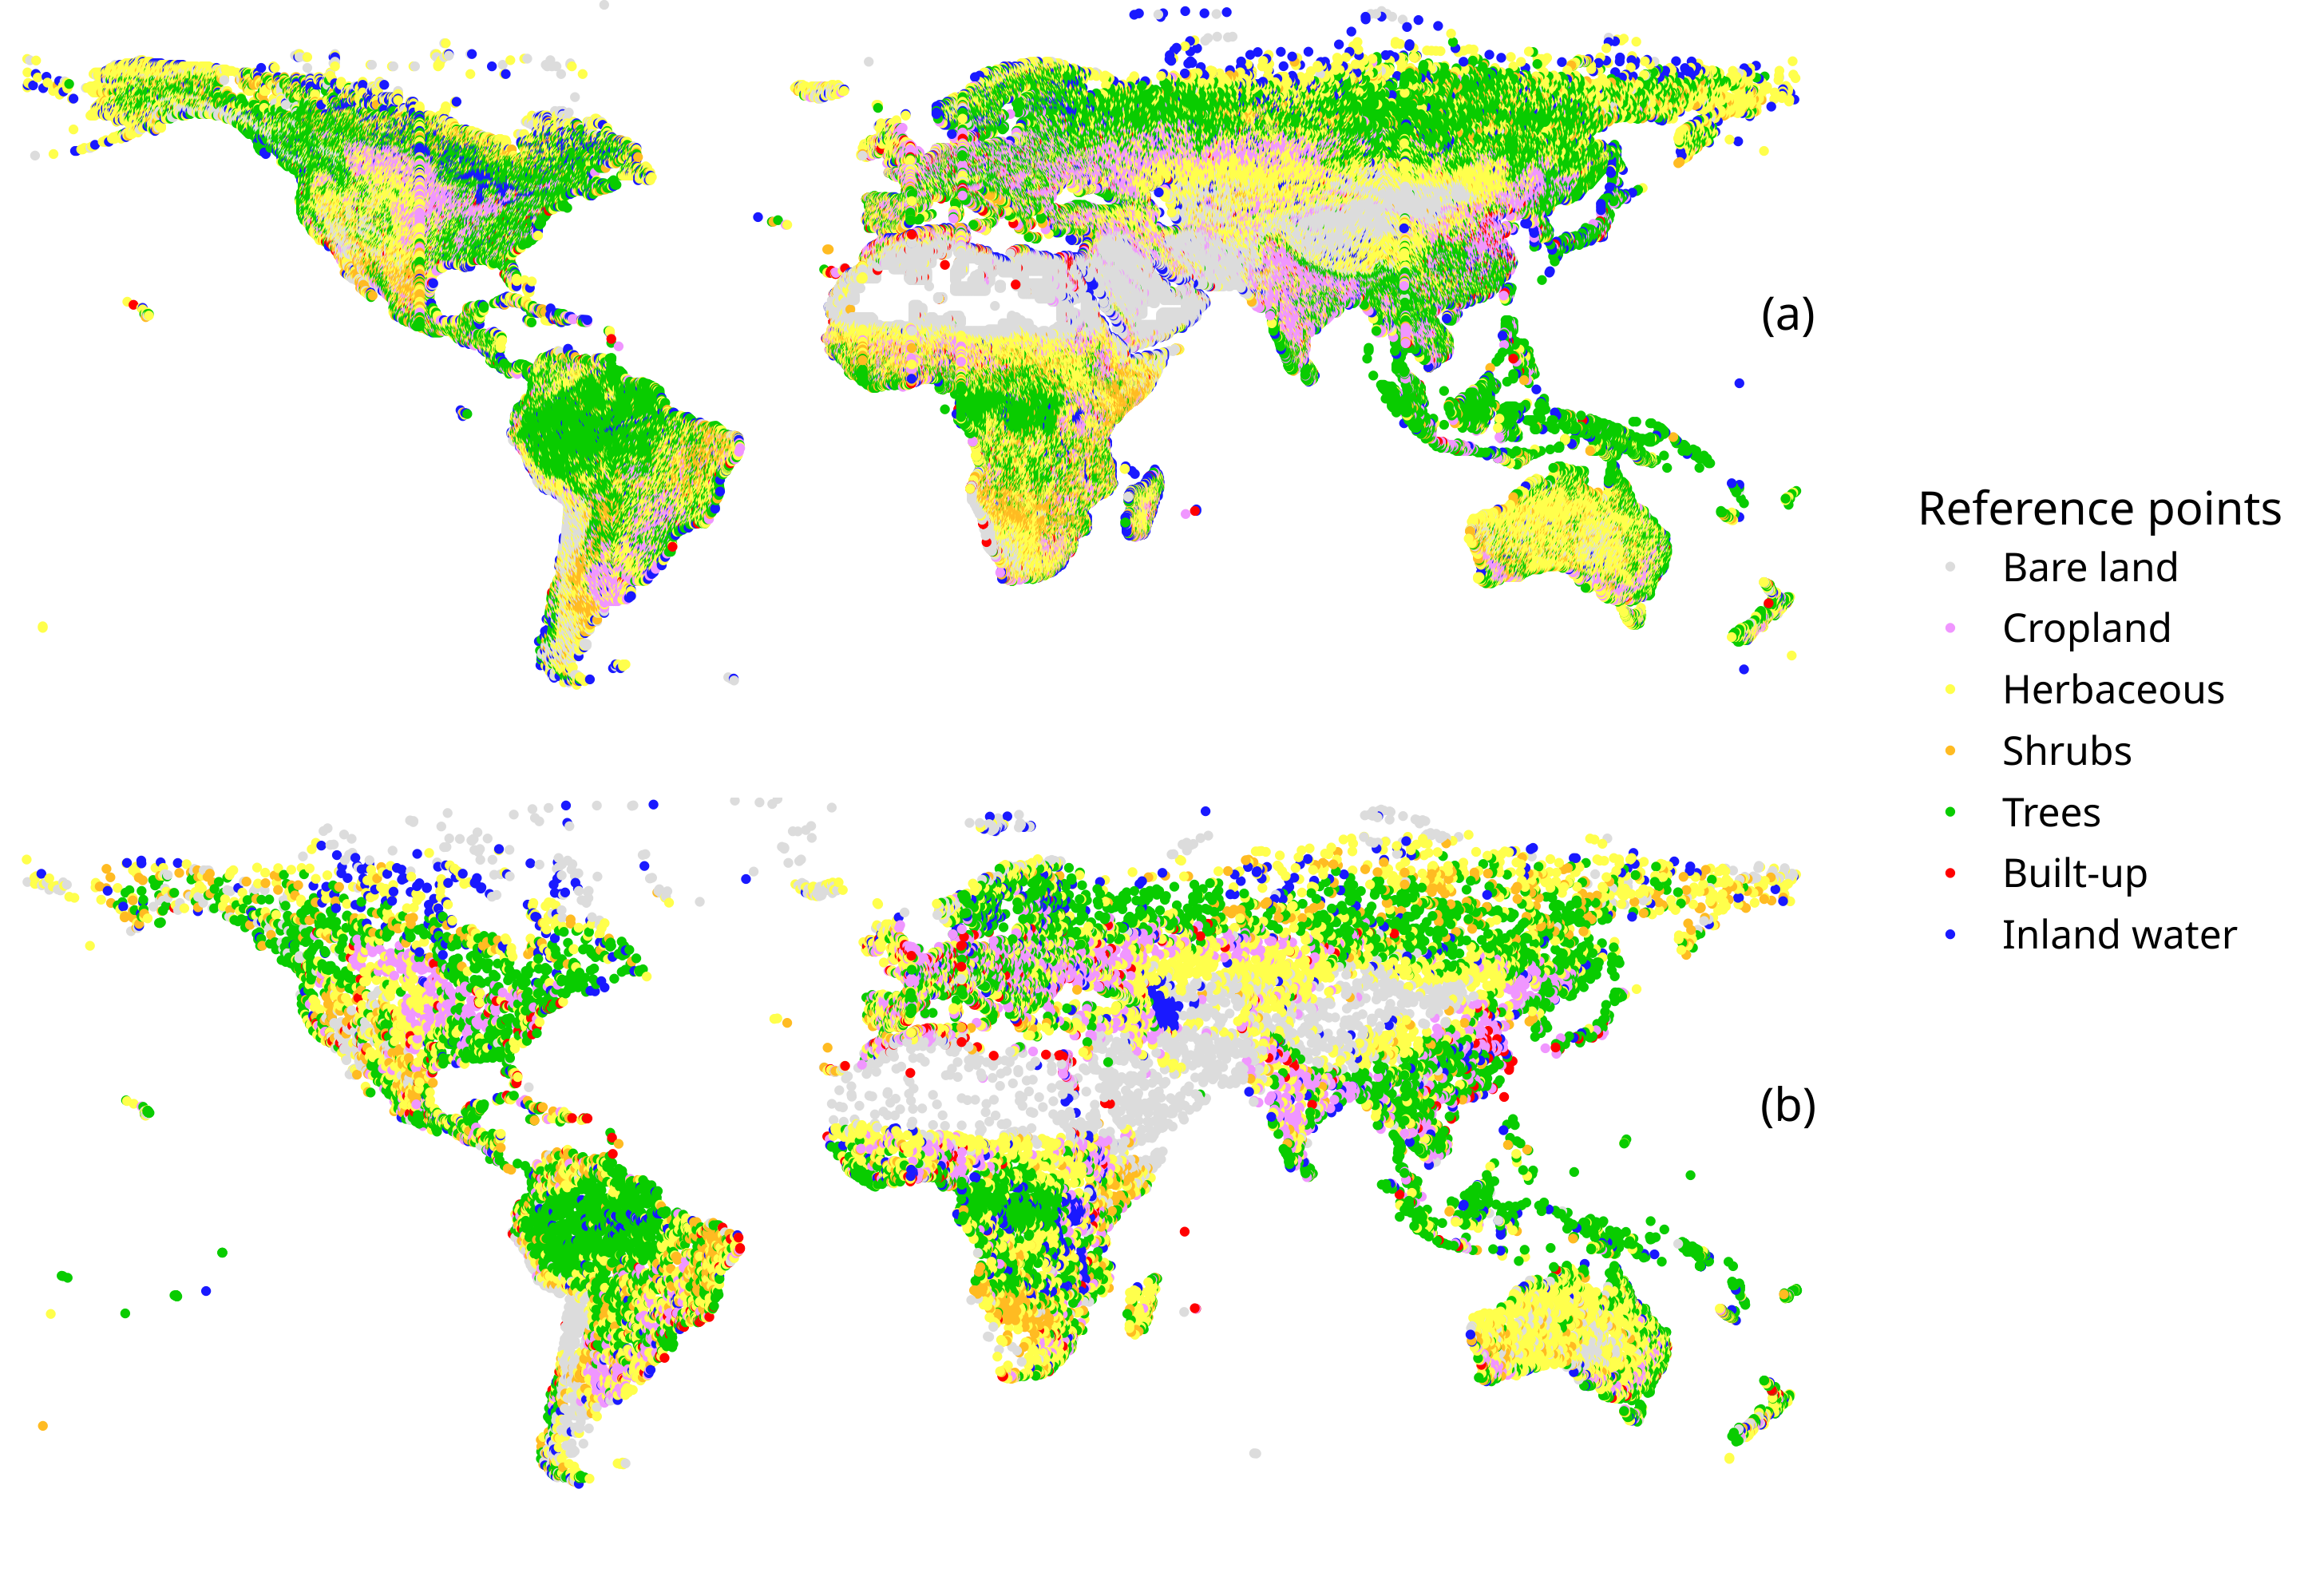
\includegraphics[width=\textwidth]{article/article-figures/maps/2020-07-06-training-and-validation}
 \caption{Sample points representing 100x100 m areas at which land cover reference data was used in the study. The colours represent the dominant land cover class at each point. (a): training dataset, collected by \gls{IIASA}, 138\,164 points used in this study. (b): validation dataset, collected by \gls{WUR}, 20\,705 points used in this study. Both datasets were collected as part of the \ac{CGLS-LC100} project \citep{buchhorn_copernicus_2020}.}
 \label{fig-reference-data}
\end{figure}

\subsection{Model covariates}

To predict land cover fractions in unsampled areas, the models learn from covariates present at the locations of the training data, and then the covariates are used for prediction in unsampled areas.
See figure \ref{fig-processing} for an overview of the whole processing chain.

In this study, six groups of covariates were used: vegetation indices, temporal metrics, terrain metrics, soil metrics, climate metrics and location data (see table \ref{tab-inputdata}).
All of these covariates had to be preprocessed before they could be input into the models.

\begin{figure}
 \centering
 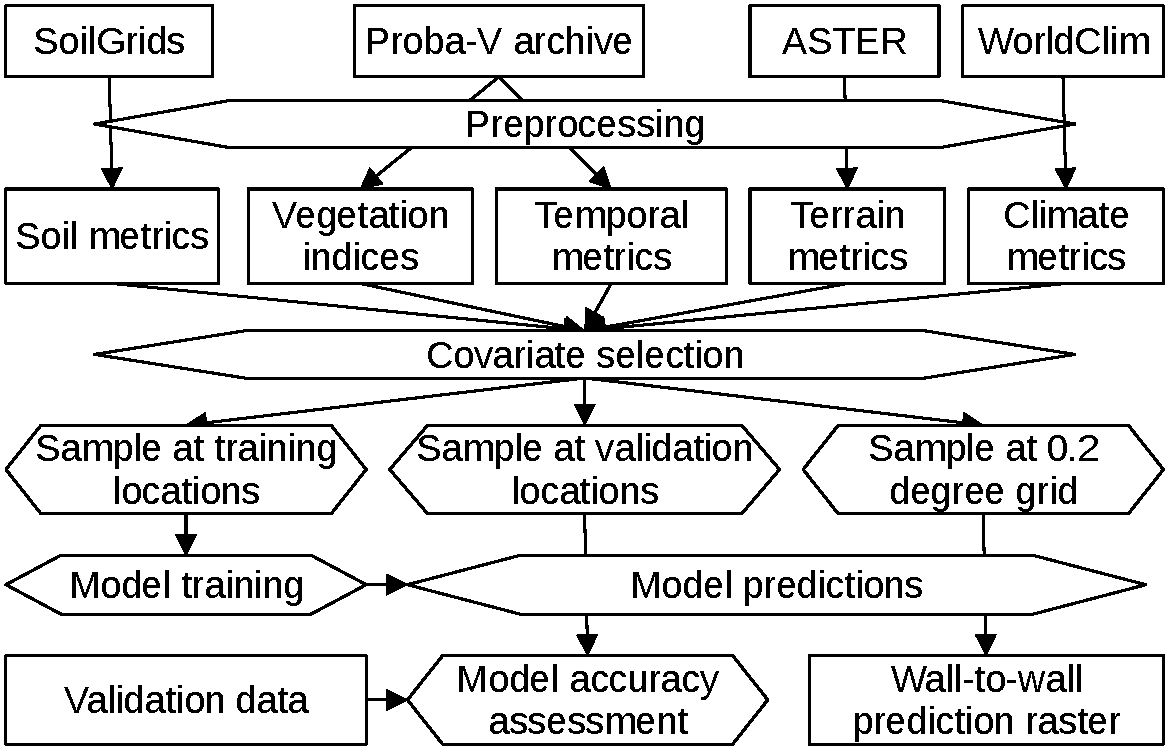
\includegraphics[width=0.75\textwidth]{article-figures/flowcharts/2020-07-10-flowchart}
 \caption{Processing workflow, from the raw input data to model accuracy assessment and wall-to-wall map output.}
 \label{fig-processing}
\end{figure}

% \begin{table}
% \centering
%     \begin{tabular}{llp{6cm}}
%          \toprule
%          \textbf{Category} & \textbf{Number} & \textbf{Data source} \\
%          \midrule
%          Spectral & 22 & PROBA-V 100m \ac{TOC} reflectance v1.02 \citep{probavguide2} \\
%          Harmonic & 9 & PROBA-V 100m \ac{TOC} reflectance v1.02 \citep{probavguide2} \\
%          Terrain & 4 & ASTER GDEM V003 \citep{ASTGTM003} \\
%          Climate & 21 & WorldClim 2.0 \citep{worldclim2} \\
%          Soil & 8 & SoilGrids \citep{hengl_soilgrids250m_2017} \\
%          Location & 3 & None (intrinsic) \\
%          \bottomrule
%     \end{tabular}
%     \label{tab-inputdata}
%     \caption{Data sources for the covariates input into the model.}
% \end{table}

%\subsubsection{Vegetation indices and temporal metrics}
\label{sec-temporal-filter}

The entire archive (2014-03-11 to 2019-07-16) of the PROBA-V 100 m Level 3 Top-of-Canopy 5-day composite product \citep{dierckx2014probav,probavguide2} was used for this study.
While the reference data corresponded to the land cover at the year 2015 specifically, the whole time series of PROBA-V was chosen to obtain more robust statistics for the temporal metrics.
Land cover change is a relatively rare phenomenon and thus, according to tests performed in the making of \gls{CGLS-LC100} collection 3, is not likely to affect more than 2\% of the training points.
Nevertheless, this may result in poorer model performance compared to if reference data for each year would be available.

The time series of each of the PROBA-V spectral bands were cloud masked, first by applying the status mask provided with the product itself, and then by running a temporal cloud filter to remove the remaining outliers that were further than 2 standard deviations away from the fitted \ac{LOESS} curve over the blue reflectance band.
The resulting cloud-free time series was then used to generate the following \glspl{VI}: \gls{NDVI}, \gls{NDMI}, \gls{EVI}, \gls{OSAVI} and \gls{NIRv}. Next, the \glspl{VI} were used to calculate the descriptive statistics (median and interquartile range) over the whole time series, as well as for each phenological season separately.
Next, harmonic analysis \citep{jakubauskas2001harmonic} was run on NDVI in order to decompose the time series into sine and cosine components for two frequency orders (annual and semiannual), as well as the trend and intercept of the model.
From this, phase and amplitude for the two orders were calculated.
Lastly, the minimum and maximum of the NDVI time series was also retained as covariates.

%\subsubsection{Terrain covariates}

For elevation data, the ASTER GDEM v003 \citep{ASTGTM003} product (30 m) was resampled to PROBA-V 100 m grid and used as the elevation covariate.
In addition, \gls{GDAL} \citep{gdal} was used to calculate terrain parameters out of elevation: slope, aspect and \ac{TPI}.
%All terrain covariates were then resampled to the PROBA-V grid.

%\subsubsection{Climate covariates}

For climate data, WorldClim 2.0 30 second product \citep{worldclim2} was used.
It includes monthly temperature, precipitation, solar radiation, wind speed and water vapour pressure data.
In addition, 19 bioclimatic parameters were calculated from the data, using the dismo package \citep{dismo}.
Some additional biophysical parameters were also calculated, namely all of the climate data during the coldest, warmest, driest and wettest months of the year at each location, as well as yearly averages of each of the original parameters.

%\subsubsection{Soil covariates}

SoilGrids \citep{hengl_soilgrids250m_2017} was used for variables related to soils.
SoilGrids is based on a random forest model that predicts soil properties at various soil depths globally at a 250 m resolution.
In the creation of SoilGrids, a land cover map (based on MODIS) had been used, and so, in order to avoid circular inference, the covariates that are significantly influenced by the land cover map as detailed in \citet{hengl_soilgrids250m_2017} were excluded.
The soil taxonomy covariates were also excluded, since they are categorical derivatives from the numerical soil property data and thus do not contribute to land cover fraction prediction.

%\subsubsection{Location covariates}

The latitude, longitude and absolute latitude of the reference points were also included when training the models, so that the models could learn spatial patterns.

\subsection{Covariate selection}
\label{sec-covariate-selection}

In total, 313 covariates were generated in pre-processing.
However, many of them are collinear with one another, which prolongs training time for machine learning models and leads to unreliable coefficient estimation and increased error variance for linear models.
Thus, variable selection was used to remove collinear covariates before predicting the land cover fractions.
Covariates that had a Pearson's correlation coefficient $r$ \citep{pearson_notes_1895} above 0.9 were excluded in an iterative process.
After that, covariates with a Spearman's rank correlation $\rho$ \citep{spearman1904rank} above 0.9 were likewise excluded.

Most of the collinear covariates were soil covariates at different depths.
Therefore the 10 cm depth covariates were left in, and the other depths excluded, as long as $r$ was above 0.9.
Similarly, climate data was collinear between subsequent months. Thus January and July data was preferred, as these months represent different extremes of the year and are less correlated with other months' data.
In addition, all of the spectral bands of PROBA-V were also highly correlated with each other as well as to \glspl{VI}, so only \glspl{VI} were kept.

After the covariate selection process, 67 covariates remained.
These covariates include data from each of the covariate categories.
See table \ref{tab-inputdata} for an overview.

%\begin{figure}
 %\inputdigraph[width=\textwidth]{article-figures/algorithms}{dot}
% 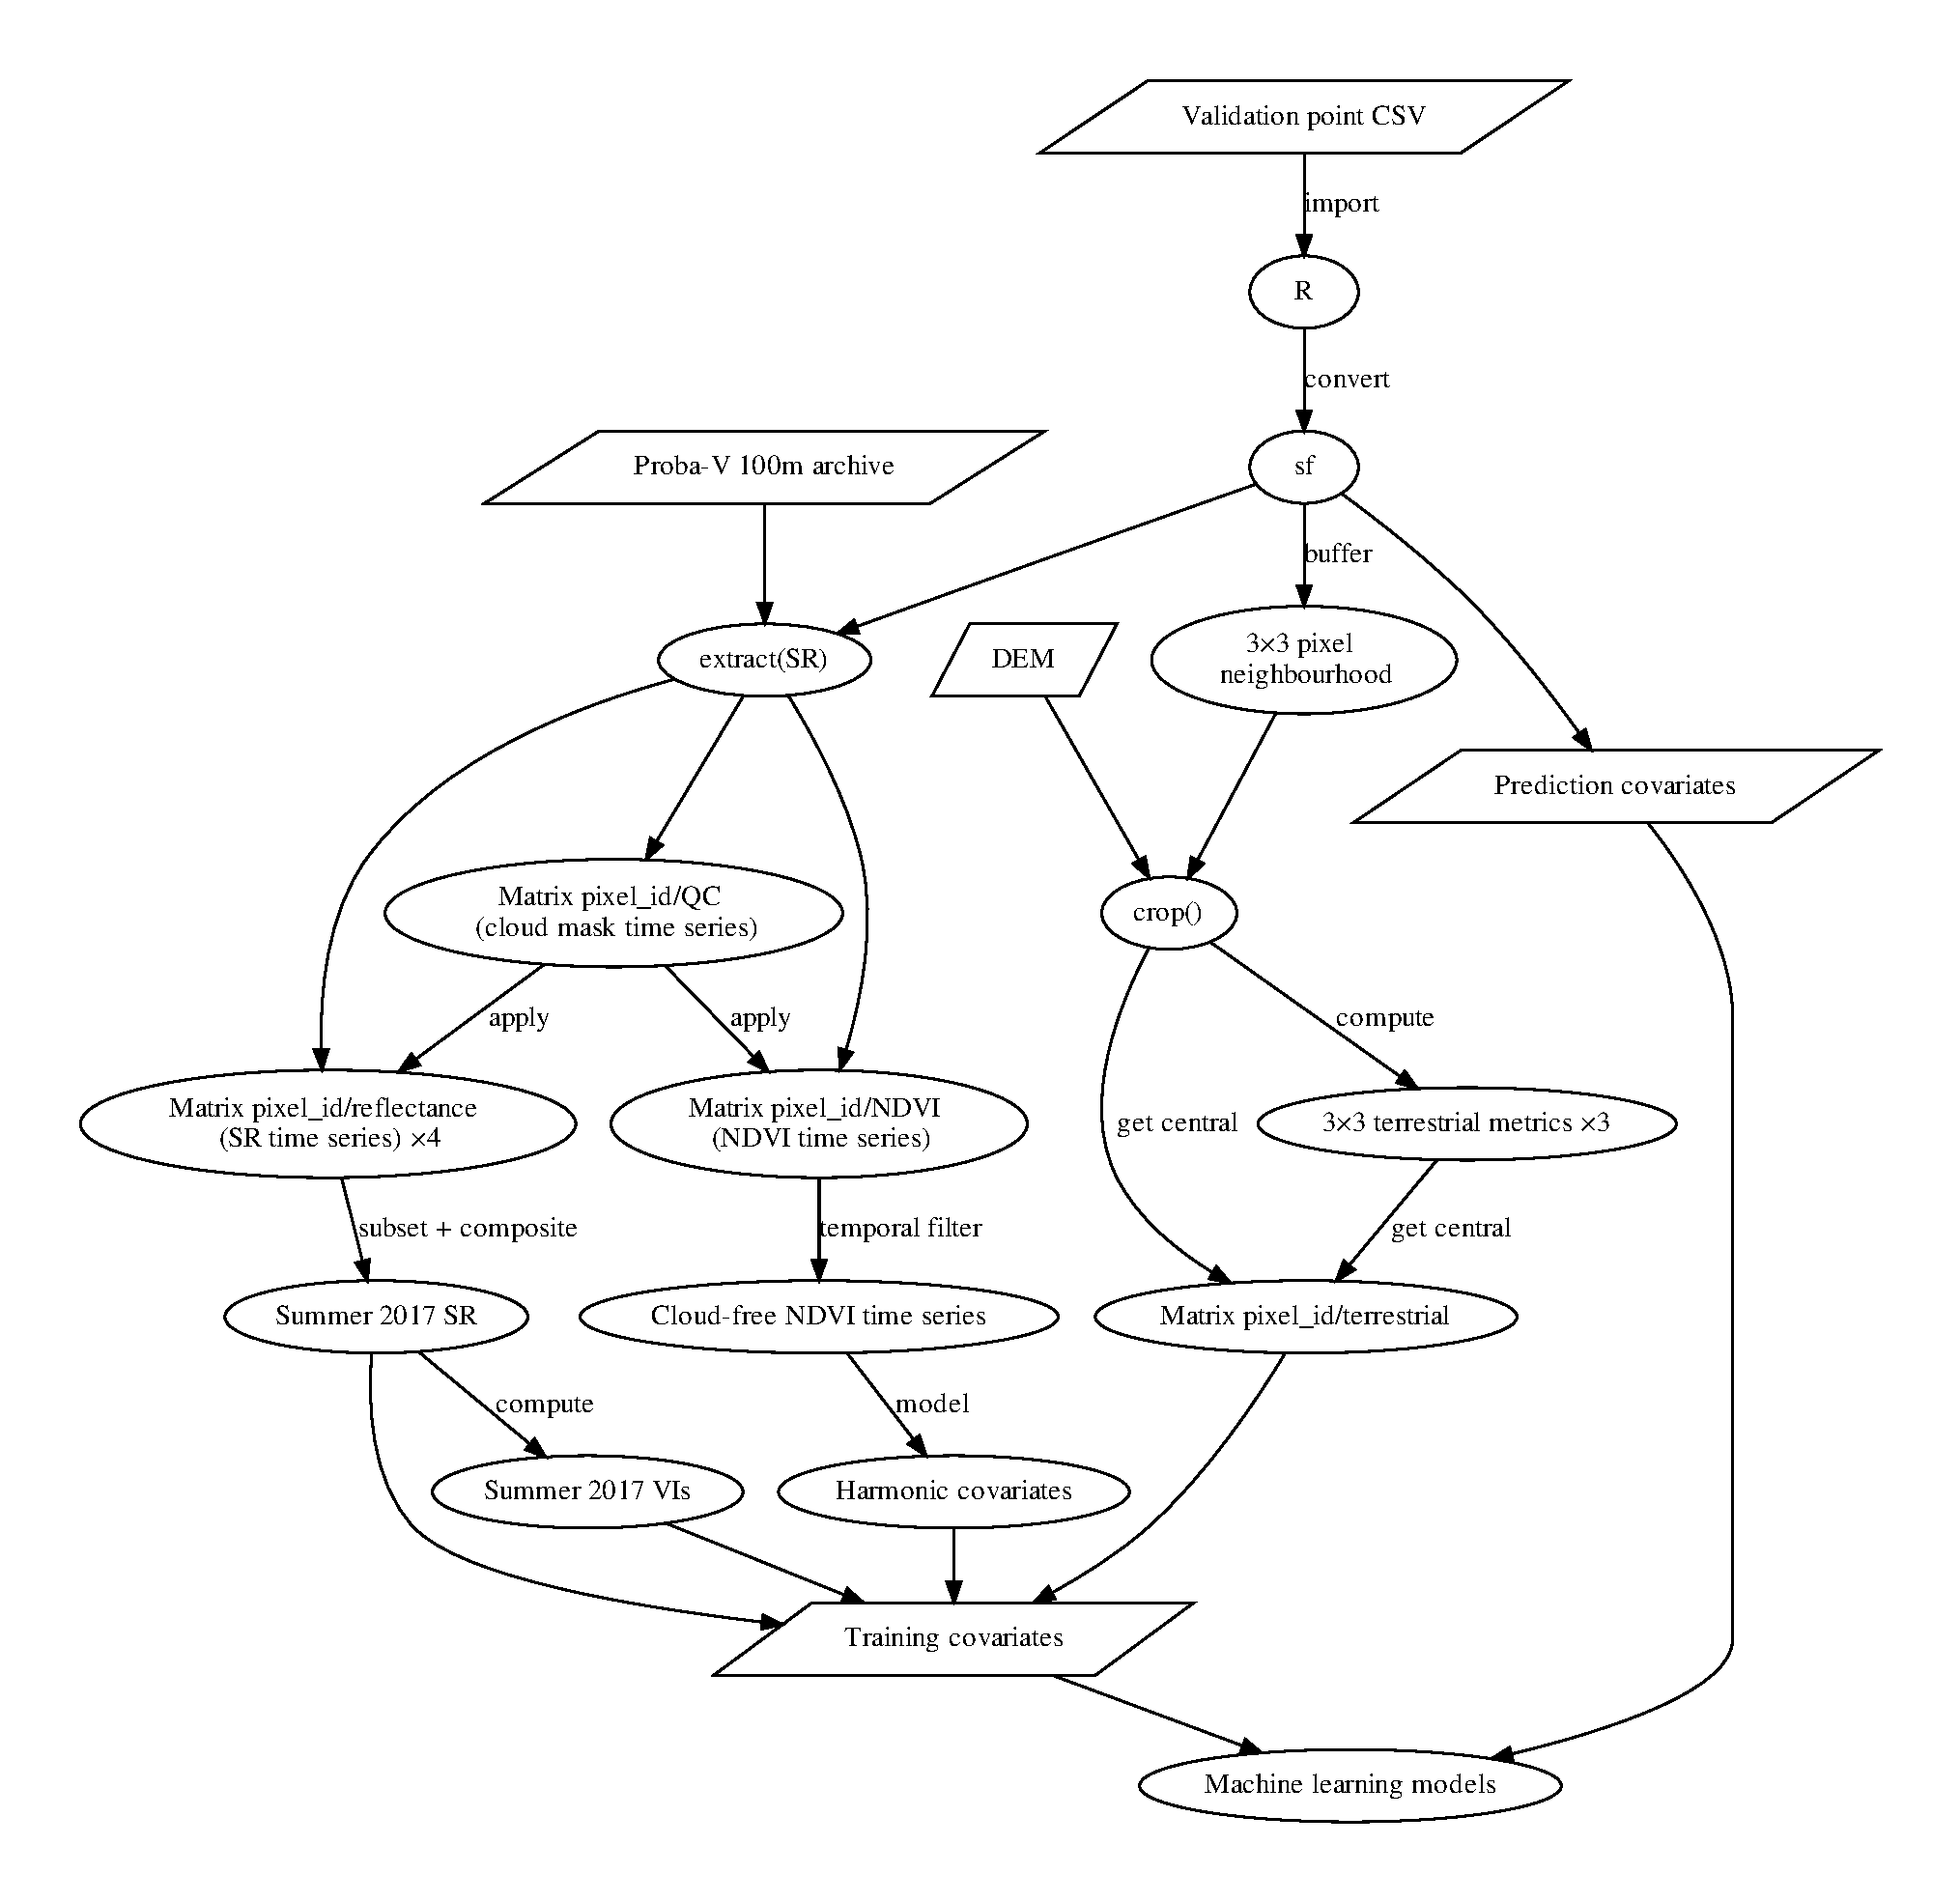
\includegraphics[width=\textwidth]{article-figures/flowcharts/algorithms}
% \caption{Preprocessing chain.}
% \label{fig-preprocessing}
%\end{figure}

\subsection{Land cover fraction mapping methods}

For deriving land cover fractions, we compared a wide array of machine learning regression methods.
We broadly divided the methods into three types: linear models, machine learning models based on \glspl{CART}, and machine learning models not based on \glspl{CART}.
See table \ref{tab-methods} for the full list of methods that were compared in this study.
%They can be broadly divided into three categories.
%Tested linear models were \ac{FNC}, \ac{GLM}, \ac{PLS} regression, Lasso regression and \ac{MLR}.
%Non-tree machine learning models tested were \ac{MLP} \glspl{NN} and \glspl{SVM}.
%Lastly, machine learning models based on \glspl{CART} tested were Cubist and \ac{RF} regressions.
In addition, as a baseline we also compared the results with an intercept model (all fractions always predicted to be equal, namely $\frac{100\%}{7}\approx14.29\%$).

All of the models were made using the free and open-source statistical software R \citep{r_2019}.

\begin{table}
\centering
    \begin{tabular}{m{4cm}ll}
         \toprule
         \textbf{Category} & \textbf{Name} & \textbf{Reference} \tabularnewline
         \midrule
         Linear models &
         \begin{tabular}{@{}l@{}}
         \Glsentryfull{FNC}\tabularnewline
         \Glsentryfull{GLM}\tabularnewline
         \Glsentryfull{PLS} regression \tabularnewline
         Lasso regression \tabularnewline
         \Glsentryfull{MLR}
         \end{tabular}
         & 
         \begin{tabular}{@{}l@{}}
         \citealt{keller_fuzzy_1985} \tabularnewline
         \citealt{neter_applied_1996} \tabularnewline
         \citealt{wold_pls-regression_2001} \tabularnewline
         \citealt{tibshirani_regression_1996} \tabularnewline
         \citealt{theil_multinomial_1969}
         \end{tabular}
         \tabularnewline \midrule
         Machine learning models based on decision trees &
         \begin{tabular}{@{}l@{}}
         \Glsentryfull{RF} regression\tabularnewline
         Cubist regression
         \end{tabular}
         &
         \begin{tabular}{@{}l@{}}
         \citealt{breiman2001random} \tabularnewline
         \citealt{cubist}
         \end{tabular}
         \tabularnewline \midrule
         Other machine learning models &
         \begin{tabular}{@{}l@{}}
         \Glsentryfullpl{MLP}\tabularnewline
         \Glsentryfull{SVM} regression
         \end{tabular}
         & 
         \begin{tabular}{@{}l@{}}
         \citealt{dreyfus_artificial_1990} \tabularnewline
         \citealt{suykens_least_1999}
         \end{tabular}
         \tabularnewline \bottomrule
    \end{tabular}
    \caption{List of regression methods for land cover fraction estimation tested in this study.}
    \label{tab-methods}
\end{table}

\subsubsection{Linear models}
%\subsubsection{\Glsentryfull{GLM}}

\Glsentryfull{GLM} \citep{neter_applied_1996}, also known as multivariate linear regression, is an extension to a regular linear regression that allows for multiple outcomes.
In this study, we used \gls{GLM} as a baseline model.
We also tested whether dropping any additional covariates from the model would result in better predictions, using a sphericity test with Greenhouse-Geisser correction to compare models with different covariates.
However, only three covariates could be dropped and it did not improve the predictions, therefore we decided to keep all the covariates in the model.
\Gls{GLM} is implemented in base R \citep{r_2019}.

%\subsubsection{Lasso/ridge/elastic net regression}

Ridge regression is a linear model regularisation method which reduces large coefficients of model covariates in order to prevent overfitting.
Lasso regression is based on the same principle, except it reduces the coefficients of each model covariate to zero if the absolute sum of coefficients is above a threshold, thus acting as a variable selection method.
Elastic net regression is a method combining the two, where model coefficients may be reduced or set to zero.
This has the effect of the coefficients of correlated covariates being set to a similar value.
We chose lasso regression \citep{tibshirani_regression_1996}, so that it would be possible to identify if there are any covariates that could be further omitted in addition to ones dropped in section \ref{sec-covariate-selection}.
The $\lambda$ parameter was chosen using cross-validation.
The lasso regression was performed using the \texttt{glmnet} package \citep{glmnet}.

%\subsubsection{\Glsentryfull{PLS} regression}

\Glsentryfull{PLS} regression \citep{wold_pls-regression_2001} is a concept related to principal component regression and also aims at reducing the input covariates into latent variables that explain the most variance of the response variable in multidimensional space.
As such, it is well suited for multicollinear data.
\ac{PLS} regression was performed using the package \texttt{pls} \citep{pls}.

All of the aforementioned linear models do not normalise the output to add up to 100\%, and also allow negative predictions.
Therefore for these models, all predictions < 0 were set to 0, and then all values were linearly rescaled per each prediction to add up to 100\%.

%\subsubsection{\Glsentryfull{FNC} regression}

\Glsentryfull{FNC} regression \citep{keller_fuzzy_1985}, also called fuzzy nearest prototype, fuzzy $c$-means or fuzzy $k$-means, is a simple regression method where the pixel's membership of a class is determined by the distance of the pixel from each class centroid in feature space.
This method always produces output that sums to 100\%.
In this study, we used an implementation adapted from the package GSIF \citep{hengl2004fuzzycmeans}.
We tested both using a logistic regression to estimate the class centroids, as well as using a weighted average of the training data to do so, and ended up using the latter method as the result was more accurate.

%\subsubsection{\Glsentryfull{MLR}}

Lastly, we tested \glsentryfull{MLR} \citep{theil_multinomial_1969}.
While logistic regressions are most commonly used for classification tasks, the output of a multinomial regression itself is the probability of a pixel to belong to each of the defined classes.
This probability can be used as a proxy for the fraction of the pixel that the class covers.
These probabilities always add up to 100\%.
However, an \ac{MLR} can only be trained on labelled data, rather than fractions.
Therefore the target (label) input for the \ac{MLR} was the name of the dominant land cover fraction of each pixel.
This does not guarantee that the pixels that the model was trained on were pure endmembers, but it allows the model to learn from a much larger dataset compared to using just the pure pixels.
The logistic regression implementation was provided by the \texttt{nnet} package \citep{nnet}.

\subsubsection{Non-tree machine learning methods}
%\subsubsection{\Glsentryfullpl{NN}}

\Glsentryfullpl{NN} are a promising technique for land cover fraction mapping, as they allow both multiple inputs and multiple outputs, and, using the softmax activation function, also ensures that the result sums up to 100\% with no need for additional postprocessing.
In this study, we used a \glsentryfull{MLP} \citep{dreyfus_artificial_1990} with three hidden layers with 128, 64 and 32 neurons per layer respectively.
Softmax activation was used to get the output.
The Nadam optimiser \citep{dozat_incorporating_2016} was used, with \gls{MAE} as the loss function.
The \texttt{keras} package \citep{keras}, built upon TensorFlow, was used as the \ac{NN} implementation, and for the ability to make use of a graphics processing unit to accelerate the neural network training process.

%\subsubsection{\Glsentryfull{SVM} regression}

\Glsentryfullpl{SVM} are machine learning models that attempt to find the optimal boundary between the class clusters in feature space by constructing a dividing hyperplane.
For land cover fraction classification, we used \gls{SVM} regression based on Least Squares \gls{SVM} \citep{suykens_least_1999}.
We used the binary relevance method, clamped the output values to the 0-100\% range and linearly scaled them to add up to 100\%.
The package \texttt{liquidSVM} \citep{liquidSVM} was suitable for this purpose, as it is optimised for processing large datasets such as ours.

\subsubsection{Tree-based machine learning methods}
%\subsubsection{\Glsentryfull{RF} regression}

\Glsentryfull{RF} regression is a popular method for land cover classification that works by building a number of \gls{CART} decision trees based on random subsets of the input training data, and taking the mean or median of the ``votes'' of these individual trees \citep{breiman2001random}.
\ac{RF} can only take one variable as the response variable, therefore there are two ways to obtain land cover fraction predictions from an \ac{RF} model.
One way is analogous to how we performed \ac{MLR}: giving labels of the dominant land cover class as the response variable, and then considering the proportion of votes from the trees as the proportions of land cover classes in the pixel.
The second way is binary relevance, where a separate model is trained to predict the presence of each class \citet{karalas2016br}.
Then the predictions are scaled linearly to sum up to 100\%.
In the case of \gls{RF}, output values do not need to be clipped as their range is always within the constraints of the input data range.
In this study, we chose the binary relevance approach, so that the model for each class would be able to learn from the fractions of all the input data, rather than just the labels of the dominant land cover class.
The processing was done using the \texttt{ranger} package \citep{ranger}.

As the results for \gls{RF} regression proved the best for \gls{RMSE}, it was also used for assessing the covariate importance.
Permutation importance was used: each covariate was shuffled in turn, and the resulting decrease in \gls{RMSE} was calculated, comparing against the validation data set.
Since the number of covariates is imbalanced by group (i.e. there are merely 3 location covariates and 22 vegetation index metrics), and there may still be colinear covariates, we also tested calculating covariate importance by permuting all covariates in a group together.
However, the result was similar to the sum of permutation importance of each individual covariates in the group, which showed that the covariate selection process had successfully eliminated all colinear covariates.
Thus we reported the more detailed covariate importance permuted per individual covariate.

%\subsubsection{Cubist regression}

Lastly, we tested Cubist regression \citep{cubist}.
It is based on \gls{RF} regression, with the major difference being that instead of using a threshold of a covariate for a split in the decision tree, Cubist instead uses a linear regression based on a subset of the data relevant for the split in question.
In addition, it features committees, a boosting technique that iteratively trains trees so as to learn from the previous ones.
For our dataset, 10 committees gave the best result.
Like with \gls{RF}, Cubist was used with the binary relevance method.
The \texttt{Cubist} package \citep{cubistpackage} was used for this.

\subsubsection{Other methods}

Additional methods were considered, but in the end turned out to be unworkable with our dataset.
Multivariate \gls{RF} is available in R provided by the \texttt{MutivariateRandomForest} package \citep{MultivariateRandomForest}, which would potentially allow better results than using regular \gls{RF} with binary relevance.
However, it is not optimised for large datasets, which did not allow to train it on more than 2000 samples at a time, making it incomparable to the rest of the tested methods.

Another model that was considered was SuperLearner \citep{SuperLearner}, an ensembling method that can combine multiple of the tested methods into one model, giving models different weights according to how well they are known to perform for a given task.
Here we ran into similar issues, as cross-validation is required for each model to train, which increases processing time dramatically.
Attempts to reduce training time by lowering the number of folds resulted in worse results than when using a single classifier.

Lastly, multiple-endmember spectral unmixing using non-negative least squares \citep{franc2005sequential} was also attempted, but the results were significantly worse than even the intercept model, possibly because the class fractions are not a linear combination of the covariates.

\subsection{Model tuning (multi-step approach) to account for value imbalance}
\label{sec-multistep}

After determining the method that performs the best, we attempted to tune it further in an attempt to solve the balance (zero inflation) problem in the training dataset.
As the dataset describes fractions of each land cover class at each point, most of the locations consist of a mix of only a few classes, and the rest of the classes are zero.
As the dataset is dominated by zeroes, minimising the objective function tends to draw the model towards predicting 0\% fractions well, and ignoring the prediction errors in the middle of the 0-100\% range.
This is not desirable for users of land cover fraction data, as the added value of fraction information is the information about the middle of the range; otherwise, discrete classification would be just as good.
Therefore we tried several approaches to increase the accuracy of the middle predictions.

For the best performing algorithm, we compared: (1) a single model, (2) a two-model approach: (a) one model to predict zeroes, and (b) one model to predict non-zeroes; and (3) a three-model approach, with (a) one model to predict pixel purity (i.e. whether we face a classification or a regression problem), (b) one to perform regression (on mixed pixels as determined by (a)), and (c) one model to perform classification (on pure pixels as determined by (a)).

%In addition, we investigated applying histogram matching, by matching the histogram of the predictions back to the histogram of the training set.
%However, that turned out to decrease accuracy in all cases, as the cases where a model predicts a value close to the true value would be set to a more extreme value to compensate for other predictions that were not as accurate to begin with.
%Therefore in the end histogram matching was not used.

\subsection{Validation/}

To assess the performance of the models, we used a number of statistical measures:

\begin{enumerate}
 \item \Gls{RMSE}, \ac{MAE}, \ac{ME}, overall and per class.
The overall measures are calculated by taking the mean of all class points pooled together, rather than taking a mean of the per-class means.
 \item \Gls{NSE} \citep{nash1970river} was used to determine the goodness of fit.
For regression output, \ac{NSE} is a method of calculating the coefficient of determination $R^2$, and is equivalent to an $R^2$ of a linear regression model whose intercept and slope terms are predetermined and are equal to 0 and 1, respectively.
 \item \Gls{SCM} \citep{silvan-cardenas_sub-pixel_2008}, and the metrics derived from it: \ac{OA}, as well as \ac{PA} and \ac{UA} per class.
The \gls{SCM} is an adaptation of the confusion matrix concept to fractional data.
When using the MIN-PROD composite operator as suggested by \citet{silvan-cardenas_sub-pixel_2008}, the diagonal of the matrix expresses the maximum overlap (agreement) of the target and predicted class fractions, and the off-diagonal is an expression of which classes the non-overlapping fractions should belong to by calculating the expected value of overlap (product of reference and predicted class fraction).
For instance, a pixel of 60\% grass and 40\% shrub, when predicted as 40\% grass and 60\% shrub, would have $min(60\%, 40\%)=40\%$ in the diagonals and $\frac{20\%\times20\%}{20\%}=20\%$ in the off-diagonals.
For cases where the allocation of the overestimated and underestimated parts of the fraction do not have a unique solution, the \ac{SCM} indicates the expected value and an associated uncertainty measure.
 \item Correlation matrix of predicted vs observed class fractions.
 \item Boxplots showing the distribution of predictions, in bins for each 10\% of the predictions, against the validation data distribution, and a comparison with the 1:1 line.
\item Lastly, spatial residuals, i.e. the overestimation and underestimation of each class fraction for each validation point, rasterised into a map.
\end{enumerate}

\section{Results}

\subsection{Method accuracy comparison}

Overall model accuracy statistics are reported in table \ref{tab-accuracy}, and per-class statistics in figure \ref{fig-models}.
\Gls{RF} regression with no adjustments (single model) obtained the lowest \gls{RMSE}, but lowest \gls{MAE} was obtained with \gls{RF} regression using the three-step model and median voting.
\gls{NSE} results follow the \gls{RMSE} results, and the \gls{OA} from the subpixel confusion-uncertainty matrix follow the \gls{MAE} results.
This is due to the \gls{NSE} being a representation of how close the data is to the 1:1 line with the validation data, where big outliers have a large effect on the value.
The \gls{SCM} does not take this into account, as it does a comparison on the overlap of fractions in each pixel, which doesn't apply an extra penalty for large errors.

\begin{table}
\centering
\begin{tabular}{llllll}
\toprule
\textbf{Model} & \textbf{\ac{RMSE} (\%)} & \textbf{\ac{MAE} (\%)} & \textbf{\acrshort{NSE}} & \textbf{\ac{OA} (\%)} & \textbf{Kappa} \\
\midrule
Intercept
& 29.9  & 21.4  & 0     & 26±5  & 0.13±0.07 \\
\Gls{FNC}
& 24.4  & 13.5  & 0.33  & 53±4  & 0.42±0.06 \\
\Gls{GLM}, \Gls{PLS}, Lasso
& 21.6  & 12.7  & 0.48  & 56±4  & 0.43±0.05 \\
%Lasso regression
%& 21.4  & 12.6  & 0.49  & 56±4  & 0.43±0.05 \\
\Gls{MLR}
& 21.6  & 12.1  & 0.48  & 58±4  & 0.46±0.06 \\
%Multivariate RF
%& 18.7  & 10.0  & 0.61  & 65±3  & 0.55±0.05 \\
\Glspl{NN}
& 22.7  & 9.2   & 0.43  & 68±1  & 0.57±0.02 \\
\Gls{SVM} regression
& 20.7  & 8.9   & 0.52  & 69±2  & 0.58±0.03 \\
Cubist regression
& 18.1  & 8.1   & 0.63  & \textbf{72±2}  & 0.63±0.03 \\
\Gls{RF} regression
& \textbf{17.3}  & 9.4   & \textbf{0.66}  & 67±4  & 0.57±0.05 \\
%\ensuremath{''} histogram matched
%& 22.0  & 9.7   & 0.43  & 66±2  & 0.58±0.03 \\
{''} RS-only
& 18.4  & 10.3  & 0.62  & 64±4  & 0.54±0.05 \\
\ensuremath{''} two-step
& 19.9  & 8.2   & 0.56  & 71±2  & 0.62±0.02 \\
\ensuremath{''} three-step
& 19.4  & 8.4   & 0.58  & 71±3  & 0.62±0.04 \\
\ensuremath{''} median vote
& 20.7  & \textbf{7.9}   & 0.52  & 71±1  & 0.63±0.02 \\
\ensuremath{''} \ensuremath{''} two-step
& 20.0  & 8.1   & 0.54  & \textbf{72±1}  & 0.63±0.02 \\
\ensuremath{''} \ensuremath{''} three-step
& 20.2  & \textbf{7.9}   & 0.54  & \textbf{72±2}  & \textbf{0.64±0.02} \\
%\ensuremath{''} \ensuremath{''} histogram matched
%& 21.3  & 9.1   & 0.46  & 68±3  & 0.61      \\
\bottomrule
\end{tabular}
\caption{Accuracy statistics of the models tested. Best performing statistics are highlighted.}
\label{tab-accuracy}
\end{table}

\begin{figure}
    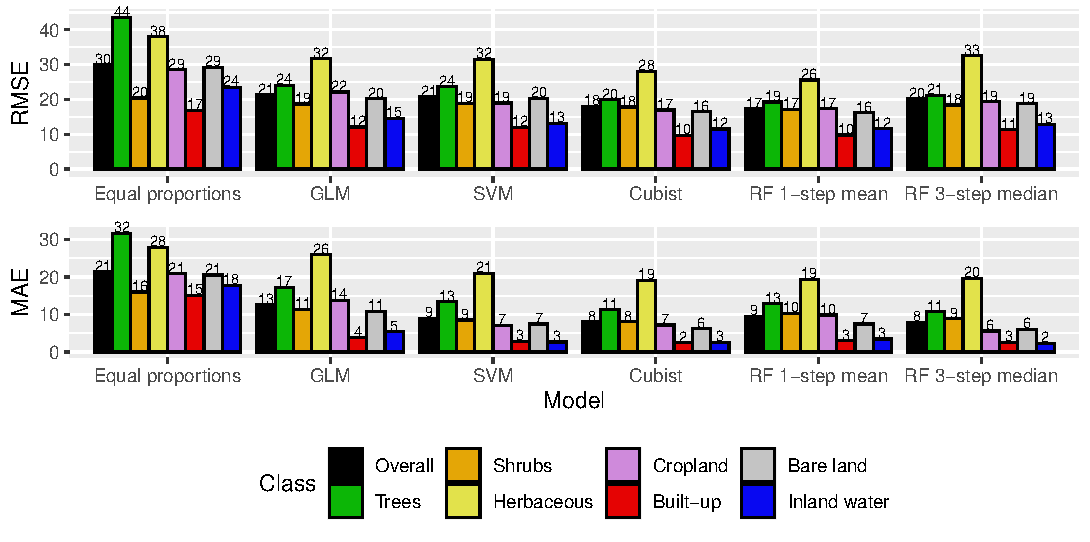
\includegraphics[width=\textwidth]{article/article-figures/barplots/2020-06-03-model-comparison-bar}
    \caption{Comparison of \gls{RMSE} (top) and \gls{MAE} (bottom) per class of the best performing models in their category, and the intercept-only model as a reference.}
    \label{fig-models}
\end{figure}

The models that performed the best (\gls{RF} and Cubist) are related models based on \gls{CART} ensembles.
Predictions per class were made using the binary relevance method (one model per class), as these models are univariate.
This shows that despite the binary relevance limitations of each model only being aware of its relevant class and not the others, and requiring a rescale step to make sure the fractions sum up to 100\%, the advantages of these machine learning models outweigh the disadvantages of the binary relevance method.

Multivariate linear statistical models (\gls{GLM}, \gls{PLS}, Lasso regression and \gls{MLR}) performed significantly worse, as they are limited to a linear approach.
The results of all of the linear models were very similar, which shows that there was no added value in \gls{PLS} and Lasso extensions over the basic \gls{GLM}.
This may be due to the additional preprocessing step of covariate selection as detailed in section \ref{sec-covariate-selection}.
It resulted in all remaining covariates being important enough to the prediction of land cover fractions, so that removing any more of them hurts rather than improves model performance.

\Gls{FNC} was the model that performed the worst out of the non-trivial models tested.
This indicates that the shape of the covariate data in feature space is too complex to capture merely with a centroid approach.
This is further evidenced by a much better result obtained by the binary relevance \gls{SVM} model, which works on a similar principle but can capture more complex shapes.

\Gls{MLP} \glspl{NN}, despite being a multivariate machine learning model, performed worse than all of the tested binary relevance methods, but better than all of the multivariate linear models.

There was a trade-off between optimisation for \gls{MAE} and \gls{RMSE}, i.e. between penalising for large misclassifications or not.
Models that had lower \gls{MAE} were more crisp, whereas models with lower \gls{RMSE} were more fuzzy.
Models that achieved lowest \gls{MAE}, in cases of high uncertainty tended to predict 100\% fractions more often, but risk misclassification, whereas models with lowest \gls{RMSE} would predict a mix of all classes that could be within the pixel, thus more often being partially but not completely wrong.

All tested models had difficulty discerning the vegetation classes (grassland, trees, crops, shrubs) between each other, and less so with the non-vegetated land cover (water, urban, bare soil), as shown in figure \ref{fig-models}.
This was exacerbated by the imbalance in class distribution: the urban class is simple to predict well due to the fact that it is rare and very rarely forms a majority, therefore a guess of 0\% is usually a good one.
In contrast, the tree fraction has a lot of samples with 100\% fraction and it deviates a lot per each sample, making it a highly unpredictable class from the data alone.
Most models showed good improvement in predicting tree cover compared to the intercept model, indicating that the covariates used were useful in distinguishing tree cover from other classes and quantifying its proportion in the pixel.
In contrast, there were only moderate improvements for predicting the grass fraction, as it is difficult for the classifiers to distinguish this class with the given input covariates.

\subsection{Adjustment for zero inflation}

Since \gls{RF} regression resulted in the lowest RMSE, it was used for testing the effect of the multi-step approach detailed in section \ref{sec-multistep}.
The overall results can be seen at the bottom of table \ref{tab-accuracy}.

\begin{figure}
    \centering
    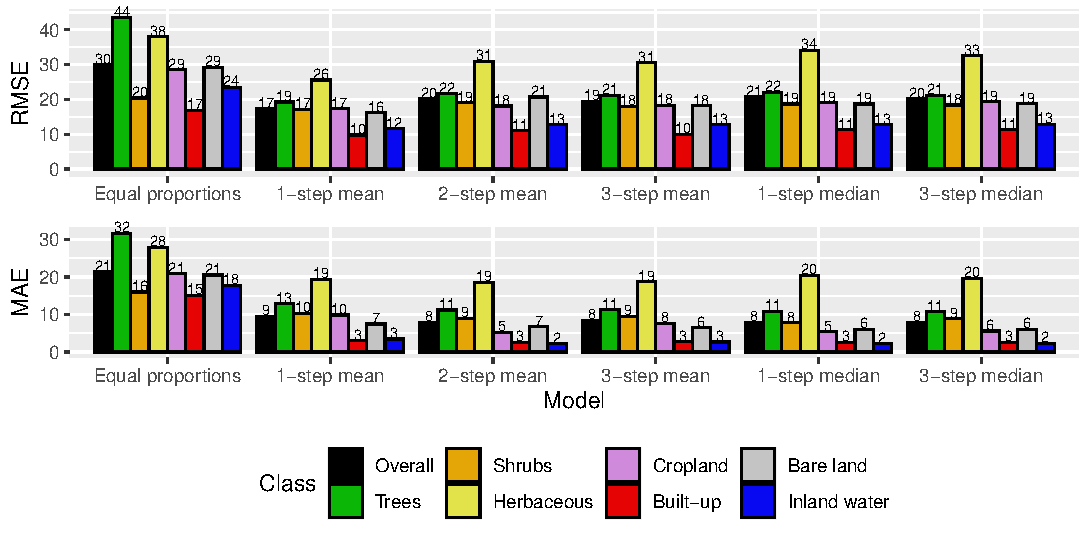
\includegraphics[width=\textwidth]{article/article-figures/barplots/2020-06-04-rf-comparison-bar}
    \caption{Comparison of \gls{RF} regression models (intercept model shown as a reference). 1-step models use no adjustment for zero inflation, 2-step models perform classification on zeroes and regression for non-zeroes, 3-step models perform a classification into pure and non-pure pixels, and then a regression or classification based on that. Mean and median are the tree vote summary statistics.}
    \label{fig-randomforest}
\end{figure}

For a \gls{RF} regression when the mean of all tree votes was used as the indicator for the land cover fraction, using a two-step approach improved the \gls{MAE} of the model, while increasing \gls{RMSE} (see figure \ref{fig-randomforest}).
This is because the false positives in the first step of the two-step model (the binary zero/non-zero classification) result in some high fractions nevertheless being set to zero.
But on average it does improve the accuracy, since without this adjustment, \gls{RF} regression would almost never assign the precise value of 0\% to a fraction, and thus result in some error for all pixels.
With this adjustment, it is possible to predict the result perfectly in the cases where the fraction is 0\%, which is the most common case.

However, the two-step approach combined with binary relevance also introduced a drawback in that there were cases where all land cover class fractions were predicted to be 0\% in the first step.
In such cases it was not possible to determine the land cover fractions, and to make them sum up to 100\%, they were all set to equal parts ($100\% / 7$), which introduced further error.

The three-step approach solved this issue, since the first step would not predict zeroes but rather purity.
In the case of pure pixels, they would be passed to \gls{RF} classification, which would always return the most likely pure class.
For mean vote \gls{RF}, the result was not significantly different from the two-step approach.
While this approach improved also the case of predicting the 100\% fractions precisely, the addition of another model caused extra error that would propagate through the process, negating the gain.

Another option explored for dealing with the issue of zero inflation was to use the median of all tree votes in \gls{RF} instead of the mean.
This had a comparable effect to using the multi-step approach, as it resulted in a lot more precise predictions for fractions with 0\%.
However, in the cases with high uncertainty, the median vote was much more likely to predict a 100\% fraction, and thus was also more likely to misclassify a pixel completely.
Thus it resulted in much higher \gls{RMSE} and much lower \gls{MAE}.
Using a multi-step approach together with median vote resulted in little difference, as the two approaches have a similar effect.
The three-step approach was an overall improvement to the single-step approach, albeit a small one.

\subsection{Covariate importance}

\Gls{RF} permutation importance was performed to test which variables were important for \gls{RF} regression predictions.
The single-step \gls{RF} model was selected for this as it achieved the lowest \gls{RMSE}.
The results are shown in figure \ref{fig-varimp}.

\begin{figure}
    \centering
    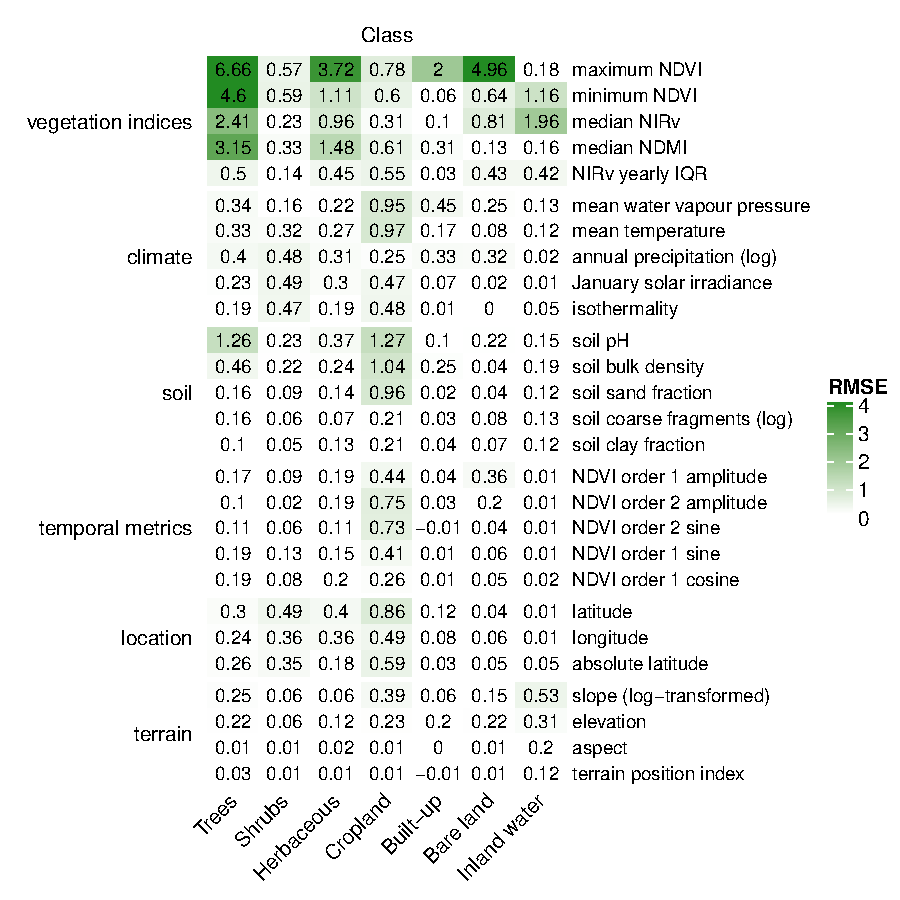
\includegraphics[width=14cm]{article-figures/heatmaps/2020-06-19-varimp-heatmap-top5}
    \caption{Random Forest single model variable importance, top 5 covariates per category. Categories are ordered by cumulative importance. The values represent decrease in RMSE when the covariate is permuted.}
    \label{fig-varimp}
\end{figure}

The overall most important variables were the maximum and minimum NDVI over the whole time series of PROBA-V imagery.
They were followed by the median NDMI and NIRv over the whole time series.
These vegetation indices were of lower importance only for the shrub and crop classes.
These two classes are complicated to distinguish from other natural vegetation, and thus benefited from a wide variety of additional covariates, including location and climate information.

To distinguish crops in particular, soil information such as pH, bulk density and sand fraction was useful for the model.
Crops are usually grown in fertile soils that can sustain them, and due to the fact that cropland is further managed, the soil is also altered to be more fertile, which affects these soil properties.
In addition, the crop prediction model benefited from harmonic metrics derived from time series the most.
The second order amplitude and sine of the harmonic model of the time series allows the model to detect areas with a double harvest throughout the year, which is indicative of crops.

Climate data was also most useful for predicting crops, especially the mean temperature and the closely (exponentially) related mean of water vapour pressure.
All of the natural precipitation class predictions benefited from (log-transformed) annual precipitation, solar irradiance in January and isothermality.

Location data was most useful for crop prediction, and to a lesser extent for grassland, shrubland and tree prediction.
These classes tend to be spatially clustered into large areas.
In contract, location information was not useful for inland water prediction as it is a rare class that takes little area.
Both absolute and regular latitude was useful for the prediction, and latitude was more useful than longitude for the predictions.

Terrain information was the least useful covariate category.
It was most useful for crops and water, as crops are inconvenient to grow on slopes or in high altitudes.
Aspect and \gls{TPI} were only useful for the water class, as standing water has no aspect and a \gls{TPI} of zero, as it has a slope of zero too.

\subsection{Spatial predictions and accuracy}

We used the single-step \gls{RF} model to predict the land cover at a global scale to obtain wall-to-wall global land cover fraction maps.
See figure \ref{fig-walltowall} for a visualisation (sampled at 0.2 degrees) of all the fraction layers combined.
The wall-to-wall fraction maps reveal how land cover fraction mapping is capable of expressing gradients and mixed land cover.

% \begin{figure}
%     \centering
%     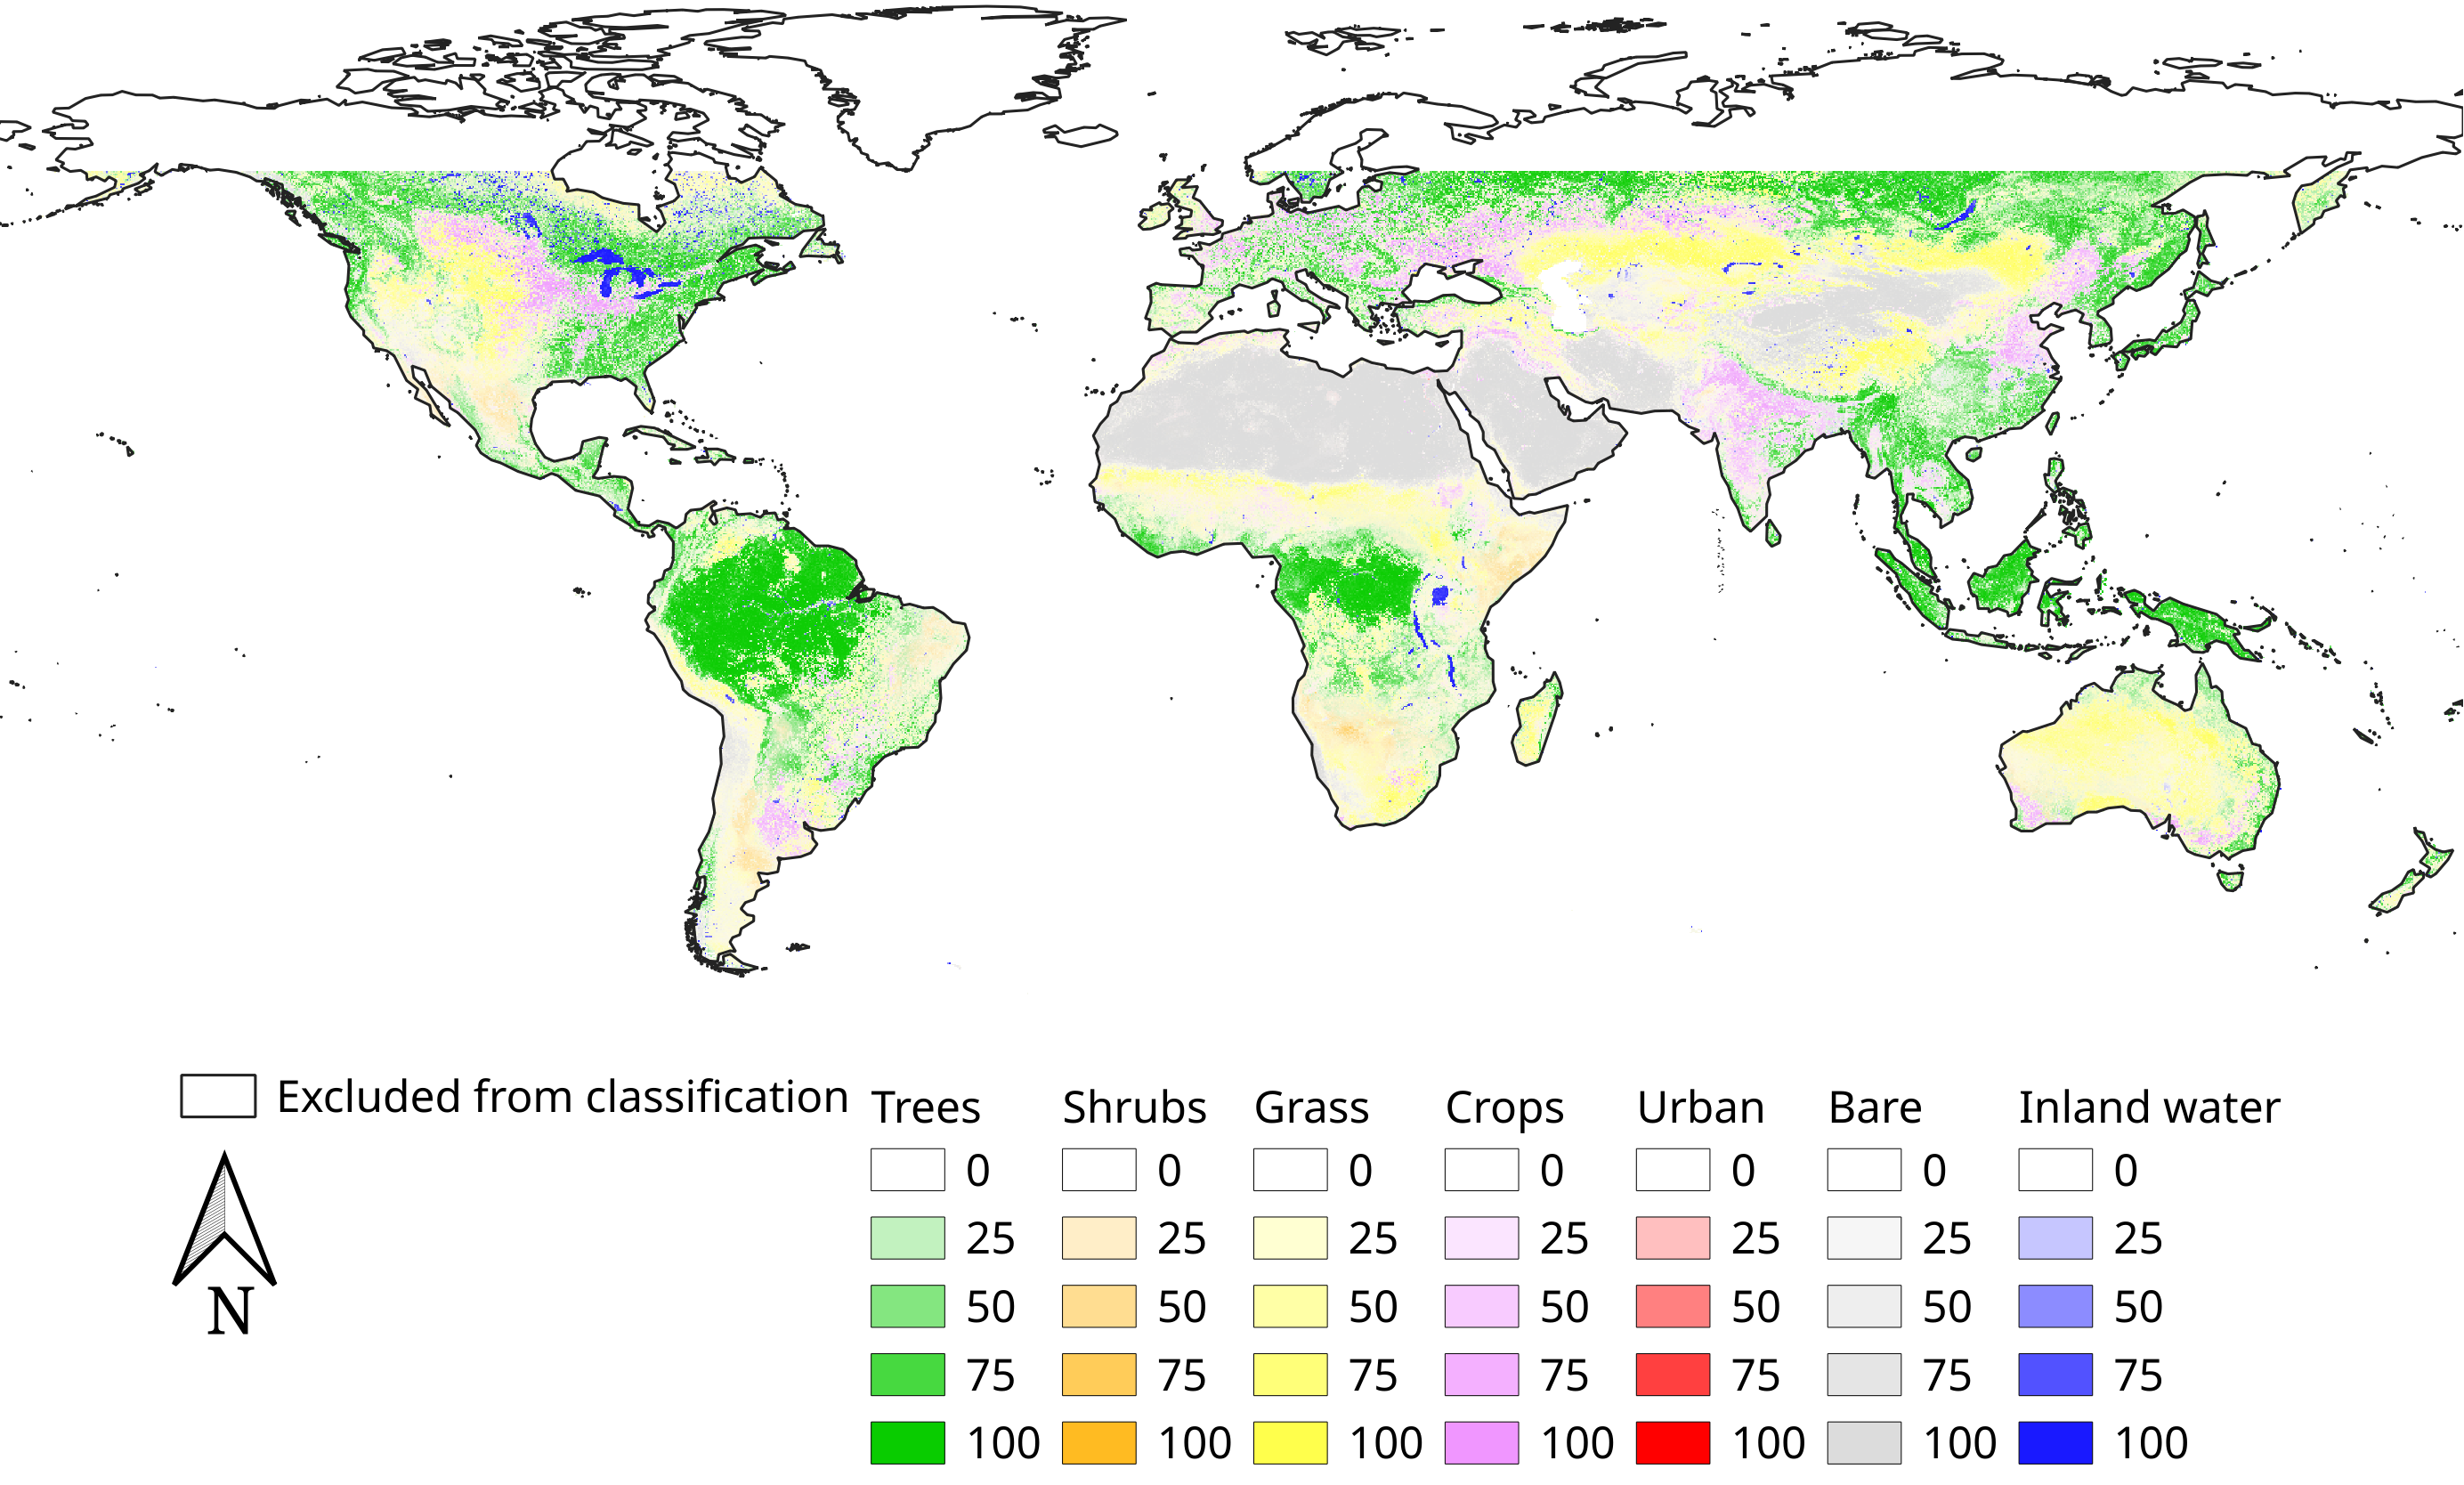
\includegraphics[width=\textwidth]{article-figures/maps/2020-05-25-walltowall}
%     \caption{Wall-to-wall predictions of all seven land cover class fractions using the single-step \gls{RF} regression model.}
%     \label{fig-walltowall}
% \end{figure}

In addition, to see whether there were any patterns in the accuracy of the predictions globally, we produced spatial accuracy maps based on the predictions in locations where we had independent validation data.
This is also presented in raster format in figure \ref{fig-walltowall}.

The global patterns of the land cover fractions are shown to express biotic gradients.
For instance, gradients are visible between communities dominated by shrubs and ones dominated by herbaceous vegetation, such as in south and east Africa.
Likewise, the gradient of tree cover from 100\% in the African tropics to 0\% in the sub-Sahara region is evident.
Herbaceous cover in sub-Sahara shows an asymmetric gradient: the cover is highest at the 14th-15th latitude and decreases quickly to the north, up to the 18th latitude, but slowly to the south, until the 5th latitude.
Inland water shows up as more discrete, as it naturally forms discrete patches and mixed pixels with water are more rare.
Built-up area is relatively rare and is rarely forms a 100\% fraction, as urban areas are in most places interspersed with greenery within the footprint of the pixel.

The spatial pattern of map accuracy shows that the land cover of areas with pure land cover was the easiest to predict, such as tropical forests (100\% tree cover) and deserts (100\% bare land).
Conversely, it was more difficult to predict fractions in areas with mixed land cover, as isolating individual fractions becomes more challenging.
In addition, land cover fractions in the extreme latitudes were more difficult to predict as well.
There less training data was available, owing to the lack of high-resolution imagery for image interpretation in these areas.

The distribution of the predictions was relatively even across the whole range for herbaceous vegetation and trees, but uneven for bare land and especially built-up area.
Built-up fraction was never predicted over 65\% and thus was more often underestimating in cases where the predicted fraction was above 15\%.
The predictions of each class showed underestimation of high fractions and overestimation of low fractions, i.e. tending towards the mean.

\begin{sidewaysfigure}
    \centering
    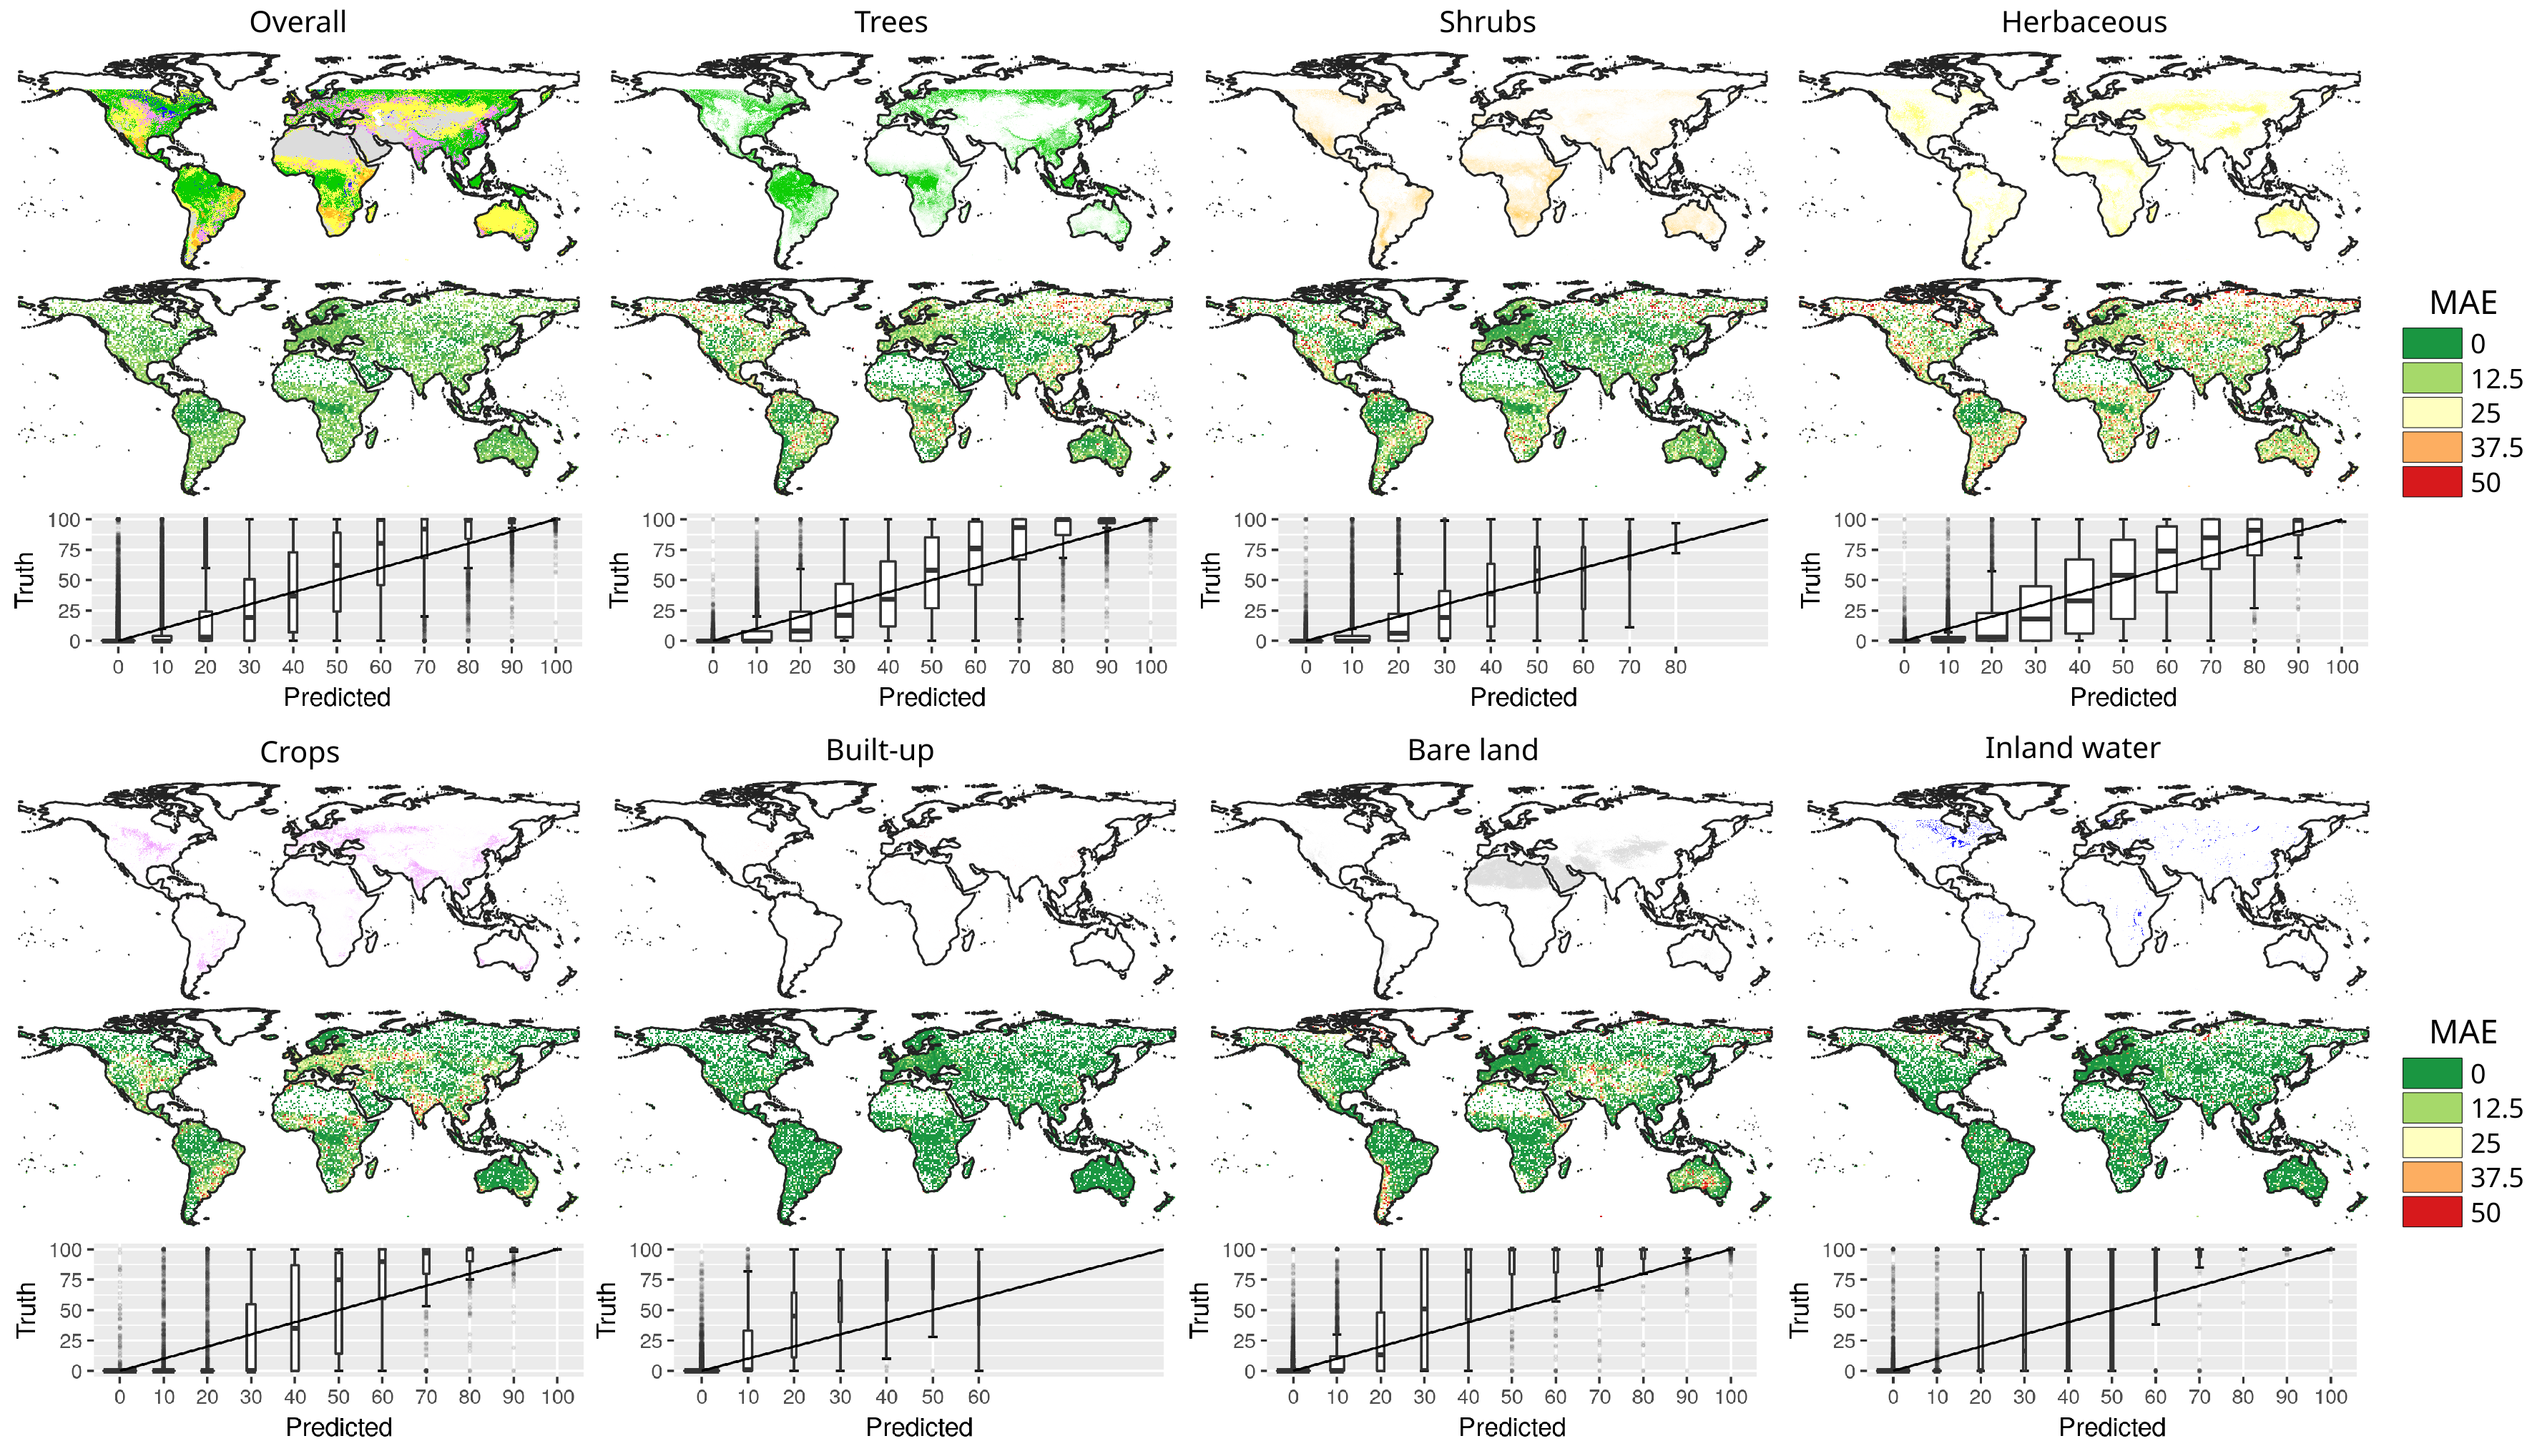
\includegraphics[width=\textwidth]{article/article-figures/maps/2020-06-19-walltowall.png}
    \caption{Random Forest single model predictions per class. Left column: predicted fractions. Middle column: absolute errors per class, based on predictions at point locations of validation data, displayed aggregated over 1 by 1 degree cells using the mean function. Right column: distribution of predicted versus true values, shown as box plots with bins each 10\%.}
    \label{fig-walltowall}
\end{sidewaysfigure}

\section{Discussion}

% \begin{enumerate}
%  \item Fraction mapping methods (Methods):
%  \begin{enumerate}
%     \item RF is the best, even though one model per class means that it does not take everything into account
%     \item Fraction area accuracy goes up to 72\%, that is good considering that hard classification is not much better than that
%     \item Hardest to classify are grasslands and especially shrubs and urban
%     \item Accuracy assessment metric makes a big difference, useful to use subpixel confusion matrix for that
%  \end{enumerate}
%  \item Optimising for zero inflation (Challenges):
%  \begin{enumerate}
%     \item Multi-step models improve MAE at the cost of RMSE and NSE
%     \item Histogram matching doesn't help any
%  \end{enumerate}
%  \item Covariate importance (Variables):
%  \begin{enumerate}
%     \item All covariates are important to a certain degree (show table of importances)
%  \end{enumerate}
% \end{enumerate}

\subsection{Methods}

In this study, we have tested a number of machine learning methods for comprehensive land cover class fraction prediction at the global scale.
Since global land cover fraction mapping is a novel field, there are few other studies or products that our results can be directly compared with.
Most products in this field are made available as layers for a particular land cover class fraction, rather than being comprehensive and guaranteeing a sum to 100\%.
In addition, the documentation for these products rarely report accuracy metrics, and none use an independent validation set for this purpose.
Lastly, these products are generated for different time scales than our study, both in terms of input time series as well as the time for which the model training data has been collected.

%The three-step Median \gls{RF} model achieved an overall accuracy of 72±2\%, which is high considering that discrete global land cover maps typically achieve around 70\% accuracy \citep{herold_challenges_2008}.
%In contrast, land cover fraction mapping is expected to be more challenging than discrete classification.
%This is because land cover fractions contain the information for all of the land cover classes considered in each pixel, and this information needs to be retrieved from discrete pixels, with no prior information about class allocation within the pixel.

Compared to a global land cover product that specialises in a specific land cover class, namely tree cover, the \gls{RF} one-step mean model had a higher RMSE (19.2\%) than the one reported by \citet{sexton_global_2013} for their vegetation continuous fields product (16.8\%).
However, the methodology for the validation differed significantly from the one used in our study, as it compared the predicted fractions to fractions as computed from lidar datasets within several local study areas, rather than using global expert image interpretation as we did.
\citet{feng_earth_2016} assessed a discrete (binary) GLCF forest cover product for three different years using a more similar methodology, and yielded similar results to ours: a user's accuracy of 98\% and producer's accuracy of 80\%, compared to the \gls{RF} three-step median tree cover user's accuracy of 81\% and producer's accuracy of 86\%.

Our results showed that \gls{RF} regression using binary relevance performed the best of all the tested algorithms.
It was also adaptive to two different goals: minimising \gls{RMSE} (default) and minimising \gls{MAE} (with median voting).
Both of these goals may be valuable to different user communities.%, depending on whether areas with high uncertainty in the predicted land cover should be treated as a mix of covers, or a guess should be made at a single most likely cover.

Compared to other studies that compared different machine learning algorithms for land cover fraction classification, we have achieved a much lower \gls{MAE}.
\citet{li_monitoring_2018} compared Cubist and \gls{RF} regression for water fraction classification and achieved \gls{MAE} as low as 7.52\% and \gls{RMSE} of 10.39\% with Cubist.
Our respective results were 2.57\% \gls{MAE} and 11.51\% RMSE.
We have confirmed that Cubist works slightly better than \gls{RF} regression for this class (\gls{RF} regression result is 11.65\% \gls{RMSE}, 3.48\% \gls{MAE}), but overall for all classes \gls{RF} regression nevertheless edges out (Table \ref{tab-accuracy}).
One important difference between the studies is that we focused on comprehensive land cover, rather than a particular class, which has an effect on the model training, and our focus was on a global rather than regional scale, has an effect on the resulting statistics due to higher sample site diversity.

Similarly, \citet{walton2008subpixelrf} assessed the accuracy of urban land cover mapping and indicated 14.5\% \gls{MAE} and 20.0\% \gls{RMSE} for Cubist, which was also observed as performing better than \gls{RF} regression and \glspl{SVM}.
Our results were 9.70\% \gls{RMSE} and 2.43\% \gls{MAE} for Cubist over the urban class, and we also observed that Cubist performed slightly better than the other two algorithms for this class.
\citet{okujeni_comparison_2014} also performed land cover fraction mapping over an urban area, but their results indicated that \gls{SVM} regression performed better than \gls{RF}.
This could be due to much finer resolution (3.6–9 m) used in their study, and the associated difference in class definitions.
The differences in the absolute numbers of \gls{RMSE} and \gls{MAE} between these studies and ours are most likely due to the different scope, namely their focus on fine scale predictions over a local area for the urban class in particular, in contrast to our global focus with comprehensive classes, leading to a different balance of the datasets between the studies.
The other studies focused on a single particular class, whereas both urban and water were relatively rare classes in our global study, and therefore the dataset had much more zero fractions in comparison, which on average is easier to predict.

\subsection{Variables}

Remote sensing variables were the most important variables in our study, especially the maximum and minimum \gls{NDVI} over the entire time series.
Note that these values are taken from a time series that has undergone temporal outlier removal, as detailed in section \ref{sec-temporal-filter}, and thus roughly correspond to the 5th and 95th percentiles of the data without additional temporal filtering.
Multiple vegetation indices were useful, with \gls{NDMI} and \gls{NIRv} median over the time series being still much more important than any other variable from other groups.
Nevertheless, even though a lot of the other covariates were of much lower importance, they  contributed to prediction accuracy enough so that they could not be easily excluded from the models as redundant (after the removal of covariates that were correlated over 0.9 as explained in section \ref{sec-covariate-selection}).
This is also due to the large variety of land cover classes in the study, since a covariate is useful if it helps predict any of the land cover classes better.
The result that including more covariates is beneficial, but remote sensing data is the most important, is in line with the conclusions of \citet{li_monitoring_2018} and \citet{hengl_soilgrids250m_2017}.
The latter study also shows high importance of climate data, however, it is focused on soils, whereas climate has more effect on soils than on land cover.
Methods based on decision trees help with effectively using covariates that may also have an overlap in the information that they provide, although linear models likewise tended to not exclude any covariates as non-informative.

\subsection{Challenges}

One challenge in land cover fraction prediction is the tendency of the models to favour the mean over the extremes, as that minimises \gls{RMSE} that may arise from incorrect predictions.
However, that leads to increased fuzziness of the result, where pixels with high uncertainty are marked as a mix of many classes, and zero fractions are rarely predicted.
Our proposed multi-step model adjusts the balance the other way round.
As it is a combination of one or two classification models and one regression model, the prediction has a lot more pure pixels compared to a single regression model.
This works very well in reducing \gls{MAE} (and improving the related metrics from the \gls{SCM}), as the especially common case of zero is captured better.
On the other hand, it comes at a cost of higher \gls{RMSE} and lower \gls{NSE}.
This is because in highly uncertain cases, the model does a best guess at a pure class, and often it is incorrect, which leads to 100\% error in those cases, which is highly penalised by \gls{RMSE}.
Due to this effect, the resulting map is closer to a discrete classification map, with less expressive transition gradients between land cover classes.
Thus we chose to present the single-model \gls{RF} regression result in figure \ref{fig-walltowall}.

A similar effect is seen when using techniques such as median vote for \gls{RF} regression.
This allows for predicting zero fractions correctly more often, but also misclassifies completely more often.
Our results showed that median vote has a stronger effect for reducing \gls{MAE} than the multi-step approach.
Combining both methods is beneficial to further reduce \gls{RMSE} for median vote predictions.

These findings show that the use of a multi-step approach depends on what is more important for the user.
If an occasional complete misclassification is acceptable, then a multi-step model provides an overall more accurate result, especially for zero fractions.
On the other hand, a single-step approach emphasises the strength of land cover fraction mapping in being able to express gradual changes over space better, and avoids large misclassifications.
We expect a multi-step approach to be more suitable for fine resolution mapping, where more pure pixels can be expected, and single-step approach to be more useful for coarse resolution mapping where mixed pixels are the norm.

Machine learning algorithms pose several challenges that are inherent to how the models are constructed.
The trade-off between minimising \gls{RMSE} and minimising \gls{MAE} comes from the chosen loss function.
In addition, the result always tends towards the mean in cases of high uncertainty.
The models predict in areas with a high cover of a fraction, such as shrublands, a lower proportion than expected, whereas in cases with a low cover, such as for fraction of built-up in dark-soil deserts, higher fractions are predicted.
This is due to a guess of the mean being less penalising than predicting the extremes incorrectly; e.g. for a case of 50\% shrub cover, predicting 100\% shrubs would be a larger mistake (and thus lead to higher RMSE) than predicting 15\% shrubs.
Likewise, predicting 0\% built-up in dark bare soils risks a case where it truly would be 100\% built-up, so on average predicting 15\% built-up in this case lowers the possible error.

There is an inherent challenge in land cover mapping for discerning classes that are related, e.g. grass and shrubs.
Grass was particularly difficult to map, in part due to confusion between grass, crops and shrubs.
These classes are similar not just to regression algorithms, but also to expert interpreters, which may lead to higher uncertainties also in the training and validation data for these classes.
Another challenge is class imbalance.
For example, the urban class is rare, it hardly ever forms a 100\% fraction and its extent small.
That makes it easy to classify, as a fraction of 0\% is in most cases a good guess, but it that makes it not useful for user needs.
This challenge is further exacerbated by the training dataset containing relatively few points in urban areas to begin with.
As such, having a more balanced training dataset may lead to a better representation of the accuracy of each class and help with class predictions.

In this study, model optimisation and dataset sizes were also a challenge.
Each model may have multiple parameters that can be tuned, and the input to each method can also be modified (e.g. by log-transforming covariates or replacing missing values).
Since the large dataset size increases the training time for the models, parameters to tune have to be chosen carefully.
As such, it is possible to miss a particular parameter combination that may further improve the results.
On the other hand, our results showed that the differences between the methods are not very high.
The differences in model parametrisations are expected to be even lower.

The scale of the study poses performance challenges, as covariates that the models use need to be available at a global scale.
Our results showed that all of the covariate groups used in the study were useful, therefore leaving a covariate out means sacrificing some predictive power.
The gain would be less time needed for processing, as that covariate would no longer need to be downloaded, preprocessed and processed.
In addition, model training performance (time for training and memory usage) may be an important consideration for global land cover mapping, as it may limit the scope of what models may be used for this task.

Several challenges are yet to be tackled in this field.
Finer spatial resolution mapping, such as 10 m mapping using Sentinel-2 data, is a future research direction, where pixels will be even more likely to be covered by a single class.
Such future developments would be more likely to benefit from a multi-model approach or optimisation for \gls{MAE}.
Alternatively, finer spatial resolution sensors would allow mapping fractions at coarser resolutions in a more precise way, as it would be possible for the model to directly make use of data from the sensor about subpixels of the mapped pixels.
Another future work direction is land cover change mapping over time.
Land cover fraction information would allow tracking gradual changes, such as regrowth, over time better.
The challenge here is that the higher uncertainty about fraction estimates may cause the time series of land cover fractions to fluctuate, making it difficult to determine trends.

\section{Conclusions}

% \begin{enumerate}
%  \item Random forest is the best
%  \item All covariates are important but to a different degree, remote sensing parameters are most important
%  \item Using a multi-model approach improves MAE at the cost of RMSE, thus a trade-off
% \end{enumerate}

In this study, we compared three groups of algorithms for land cover fraction mapping and created a demonstation map showing the result of the best performing model by \gls{RMSE}.
We also introduced a multi-step approach to tackle the issue of correctly predicting the extreme fraction values of 0\% and 100\%.
The best performing models were based on \gls{CART} tree ensembles, with \gls{RF} regression performing the best overall.
A single-step \gls{RF} regression model using majority voting resulted in the best results for RMSE (17.3\%) and \gls{NSE} (0.66).
Using median voting combined with the three-step approach obtained the best results for \gls{MAE} (7.9\%) and \gls{SCM} \gls{OA} (72±2\%).
Remote sensing covariates were the most important in the models, although all other types of covariates (climate, soil, terrain) also contributed to the model significantly.
This demonstrates the possibility of exhaustive global land cover fraction mapping using currently available methods, offering better precision than discrete land cover maps.
It also allows the users to define their own thresholds to generate discrete classifications of their own choosing, based on their classes on interest.
This work paves the way for operationalisation of global land cover fraction mapping.

% Converted from role-centric to person-centric as per Elsevier guidelines: https://www.elsevier.com/authors/journal-authors/policies-and-ethics/credit-author-statement
\minisection{Author Contributions}
\textbf{Dainius Masiliūnas}: Methodology, Formal Analysis, Software, Writing – Original Draft, Data Curation. \textbf{Nandin-Erdene Tsendbazar}: Investigation, Data Curation, Supervision, Conceptualisation, Writing – review \& editing. \textbf{Martin Herold}: Conceptualisation, Project Administration, Supervision, Methodology. \textbf{Myroslava Lesiv}: Investigation, Data Curation. \textbf{Marcel Buchhorn}: Writing – review \& editing. \textbf{Jan Verbesselt}: Conceptualisation, Methodology, Supervision, Writing – review \& editing.

% \begin{itemize}
%     \item Conceptualisation: MH NT JV
%     \item Data curation: DM
%     \item Formal Analysis: DM
%     \item Funding acquisition: JV MH BS
%     \item Investigation: DM ML NT
%     \item Methodology: DM MH JV NT BK LL
%     \item Project administration: MH NT JV
%     \item Resources: MH BS
%     \item Software: DM
%     \item Supervision: MH NT JV
%     \item Validation: NT DM
%     \item Visualisation: DM MH
%     \item Writing – original draft: DM
%     \item Writing – review \& editing: NT JV MH MB BS
% \end{itemize}

\minisection{Acknowledgements} We would like to thank VITO and Terrascope for providing us with computational facilities to access and process {PROBA-V} data, and IIASA for providing the model training dataset. In addition, we thank Benjamin Kellenberger for help on tuning neural network parameterisation, as well as Linlin Li and Tomislav Hengl for suggestions on additional machine learning methods to test.

%\minisection{Conflicts of Interest} The authors declare no conflict of interest.

%\minisection{Appendix 1} % Not sure how to typeset this, as it does not fit under the section header here.
\begin{table}
\begin{center}
\begin{adjustbox}{max width=8cm}
\begin{tabular}{m{12cm}l}
\toprule
\multicolumn{1}{l}{Category \& data source}&\multicolumn{1}{c}{Covariate}\tabularnewline
\midrule
Location (3, intrinsic)&
\begin{tabular}{@{}l@{}}longitude\tabularnewline
latitude\tabularnewline
absolute latitude
\end{tabular}\tabularnewline
\midrule
Vegetation indices (22, derived from PROBA-V 100m \ac{TOC} reflectance v1.02 \citep{probavguide2})&
\begin{tabular}{@{}l@{}}
minimum NDVI\tabularnewline
maximum NDVI\tabularnewline
median NDMI\tabularnewline
NDMI yearly IQR\tabularnewline
NDMI March-May IQR\tabularnewline
NDMI June-August IQR\tabularnewline
NDMI September-November IQR\tabularnewline
NDMI December-February IQR\tabularnewline
OSAVI March-May IQR\tabularnewline
OSAVI June-August IQR\tabularnewline
OSAVI September-November IQR\tabularnewline
OSAVI December-February IQR\tabularnewline
EVI March-May IQR\tabularnewline
EVI June-August IQR\tabularnewline
EVI September-November IQR\tabularnewline
EVI December-February IQR\tabularnewline
median NIRv\tabularnewline
NIRv yearly IQR\tabularnewline
NIRv March-May IQR\tabularnewline
NIRv June-August IQR\tabularnewline
NIRv September-November IQR\tabularnewline
NIRv December-February IQR
\end{tabular}\tabularnewline
\midrule
Temporal metrics (9, derived from a harmonic model over time series of PROBA-V 100m \ac{TOC} reflectance v1.02 \citep{probavguide2})&
\begin{tabular}{@{}l@{}}
NDVI order 1 cosine\tabularnewline
NDVI order 1 sine\tabularnewline
NDVI order 2 cosine\tabularnewline
NDVI order 2 sine\tabularnewline
NDVI trend coefficient\tabularnewline
NDVI order 1 phase\tabularnewline
NDVI order 1 amplitude\tabularnewline
NDVI order 2 phase\tabularnewline
NDVI order 2 amplitude
\end{tabular}\tabularnewline
\midrule
Terrain (4, ASTER GDEM V003 \citep{ASTGTM003})&
\begin{tabular}{@{}l@{}}
elevation\tabularnewline
slope (log-transformed)\tabularnewline
aspect\tabularnewline
terrain position index
\end{tabular}\tabularnewline
\midrule
Climate (21, WorldClim 2.0 \citep{worldclim2})&
\begin{tabular}{@{}l@{}}
January precipitation (log)\tabularnewline
April precipitation (log)\tabularnewline
July precipitation (log)\tabularnewline
October precipitation (log)\tabularnewline
January solar irradiance\tabularnewline
July solar irradiance\tabularnewline
mean temperature\tabularnewline
temperature monthly range\tabularnewline
isothermality\tabularnewline
temperature annual range\tabularnewline
annual precipitation (log)\tabularnewline
temperature seasonality\tabularnewline
minimum solar irradiance\tabularnewline
maximum solar irradiance\tabularnewline
mean solar irradiance\tabularnewline
mean windspeed\tabularnewline
mean water vapour pressure\tabularnewline
coldest month precipitation (log)\tabularnewline
warmest month precipitation (log)\tabularnewline
wettest month solar irradiance\tabularnewline
driest month solar irradiance
\end{tabular}\tabularnewline
\midrule
Soil (8, SoilGrids \citep{hengl_soilgrids250m_2017})&
\begin{tabular}{@{}l@{}}
soil available water\tabularnewline
soil bulk density\tabularnewline
soil cation exchange capacity (log)\tabularnewline
soil clay fraction\tabularnewline
soil coarse fragments (log)\tabularnewline
soil pH\tabularnewline
soil sand fraction\tabularnewline
soil water wilting point
\end{tabular}\tabularnewline
\bottomrule
\end{tabular}
\end{adjustbox}
\caption{List of covariates input into the models, and their data sources.}
\label{tab-inputdata}
\end{center}
\end{table}

%\section*{Abbreviations}

%\printnoidxglossary[type=acronym]

\bibliography{article-bib}

\end{document}
